\section{مقایسهٔ جامع همهٔ ماژول‌ها و کالبدشکافی تجربی نتایج}
\label{sec:all_modules_comparison}

این بخش کارنامه تجربی نهایی و مقایسه جامع چندمعیاره تمامی ماژول‌های توسعه‌یافته و ارزیابی‌شده در چارچوب پژوهش را ارائه می‌دهد. این ارزیابی‌ها بر مبنای \textbf{۲,۴۳۲ اجرای تجربی ثبت‌شده در لجر رسمی سخت‌افزار} بر روی کارت گرافیک \lr{NVIDIA GeForce RTX 4070 Laptop} (معماری \lr{Ada Lovelace, SM 8.9}) با ۲,۵۴۲ رکورد در پایگاه داده لجر (\lr{\texttt{results/registry/master\_ledger.sqlite}}) و \textbf{۶۲۹ ماژول حسابرسی‌شده} در ماتریس جامع نتایج (\lr{\texttt{results/MASTER\_RESULTS\_MATRIX.csv}}) استوار است.

توزیع موضوعی و کارکردی ۶۲۹ ماژول مستقل حسابرسی‌شده در جدول \ref{tab:category_distribution_persian} خلاصه گردیده است:

\begin{table}[H]
\centering
\caption{توزیع ساختاری و قلمرو عملیاتی ۶۲۹ ماژول مستقل ارزیابی‌شده در چارچوب یکپارچه پژوهش}
\label{tab:category_distribution_persian}
\small
\begin{tabular}{lcp{0.62\textwidth}}
\toprule
\textbf{دسته معماری (\lr{Category})} & \textbf{تعداد ماژول} & \textbf{دامنه کاربرد و قلمرو عملیاتی} \\
\midrule
\lr{attention} & ۴۶۷ & مکانیزم‌های توجه زیردرجه دوم، خطی، بازگشتی، حالت‌فضا، ترکیبی و خلوت \\
\lr{compressor} & ۱۰۱ & موتورهای فشرده‌سازی SVD، تجزیه هوس‌هولدر، هرس ساختاریافته و کوانتایزاسیون برداری \\
\lr{triton\_kernel} & ۴۰ & کرنل‌های کامپایل درجا در زبان تریتون برای بهره‌برداری حداکثری از حافظه سریع SRAM \\
\lr{cuda\_kernel} & ۱۸ & عملگرهای بومی بهینه‌سازی‌شده به زبان CUDA C++ با پشته گسیل سه‌سطحی \\
\lr{ablation} & ۲ & بسته‌های تحلیلی بررسی خطای تراکمی، سفیدسازی چولسکی و هوموتوپی پیوسته \\
\lr{baseline} & ۱ & مدل‌های متراکم پایه (\lr{Dense Teachers}) به عنوان سنگ‌محک استاندارد مقایسه \\
\midrule
\textbf{مجموع کل} & \textbf{۶۲۹} & \textbf{مجموعه کامل ماژول‌های حسابرسی‌شده در ماتریس جامع نتایج} \\
\bottomrule
\end{tabular}
\end{table}

مقایسه علمی ماژول‌ها باید بر اساس چهار پرسش کلیدی خوانده شود:
\begin{enumerate}
    \item \textbf{کیفیت بازنمایی زبانی:} کدام ماژول‌ها قادرند در وظایف زبانی دشوار (نظیر استدلال دوتایی \lr{MNLI} با ۳ کلاس) دقت خود را حفظ کرده و دچار فروپاشی رتبه زیرفضا نگردند؟
    \item \textbf{بهره‌وری سخت‌افزاری و حافظه:} کدام معماری‌ها موفق شده‌اند ردپای اوج حافظه \lr{(Peak VRAM)} را به حداقل رسانده و گلوگاه انتقال حافظه سراسری را برطرف سازند؟
    \item \textbf{مقیاس‌پذیری مجانبی در توالی‌های بلند:} در چه طول توالی، هزینه‌های ثابت پرتاب کرنل جبران شده و نقطه تقاطع مجانبی (\lr{Crossover Point}) نسبت به توجه متراکم استاندارد محقق می‌گردد؟
    \item \textbf{پایداری و دروازه کیفیت:} آیا ماژول موفق به اخذ تاییدیه دروازه کیفیت (\lr{PASS}) شده است یا دچار رفتارهای آسیب‌شناختی نظیر فروپاشی به رده اکثریت (\lr{Majority Class Collapse}) یا انفجار پرپلکسیتی لاجیت گردیده است؟
\end{enumerate}

\subsection{نمودارهای مقایسه‌ای و تحلیل تصویری عملکرد}
شکل‌های \ref{fig:comparison_accuracy_top15} تا \ref{fig:comparison_pass_fail} دیدی بصری و چندمعیاره از توزیع عملکرد ماژول‌های تاییدشده ارائه می‌دهند: در شکل \ref{fig:comparison_accuracy_top15} رتبه‌بندی ۱۵ ماژول برتر، در شکل \ref{fig:comparison_champion} مقایسه چندبعدی ماژول‌های قهرمان، در شکل \ref{fig:comparison_memory_reduction} میزان تقلیل ردپای اوج حافظه گرافیکی، در شکل \ref{fig:comparison_pareto_vram} جبهه بهینگی پارتو، در شکل \ref{fig:comparison_radar_families} نمودار رادار ۶ خانواده معماری، در شکل \ref{fig:comparison_heatmap} نقشه حرارتی عملکرد، و در شکل \ref{fig:comparison_pass_fail} توزیع وضعیت دروازه کیفیت به تفکیک خانواده‌ها به تصویر کشیده شده است. نمودارها بر پایه ردیف‌های دارای وضعیت \lr{PASS} بر روی مدل \lr{DistilBERT} در بنچ‌مارک \lr{SST-2} رسم گردیده‌اند تا شرط مقایسه هم‌شرط نقض نشود.

\begin{figure}[H]
\centering
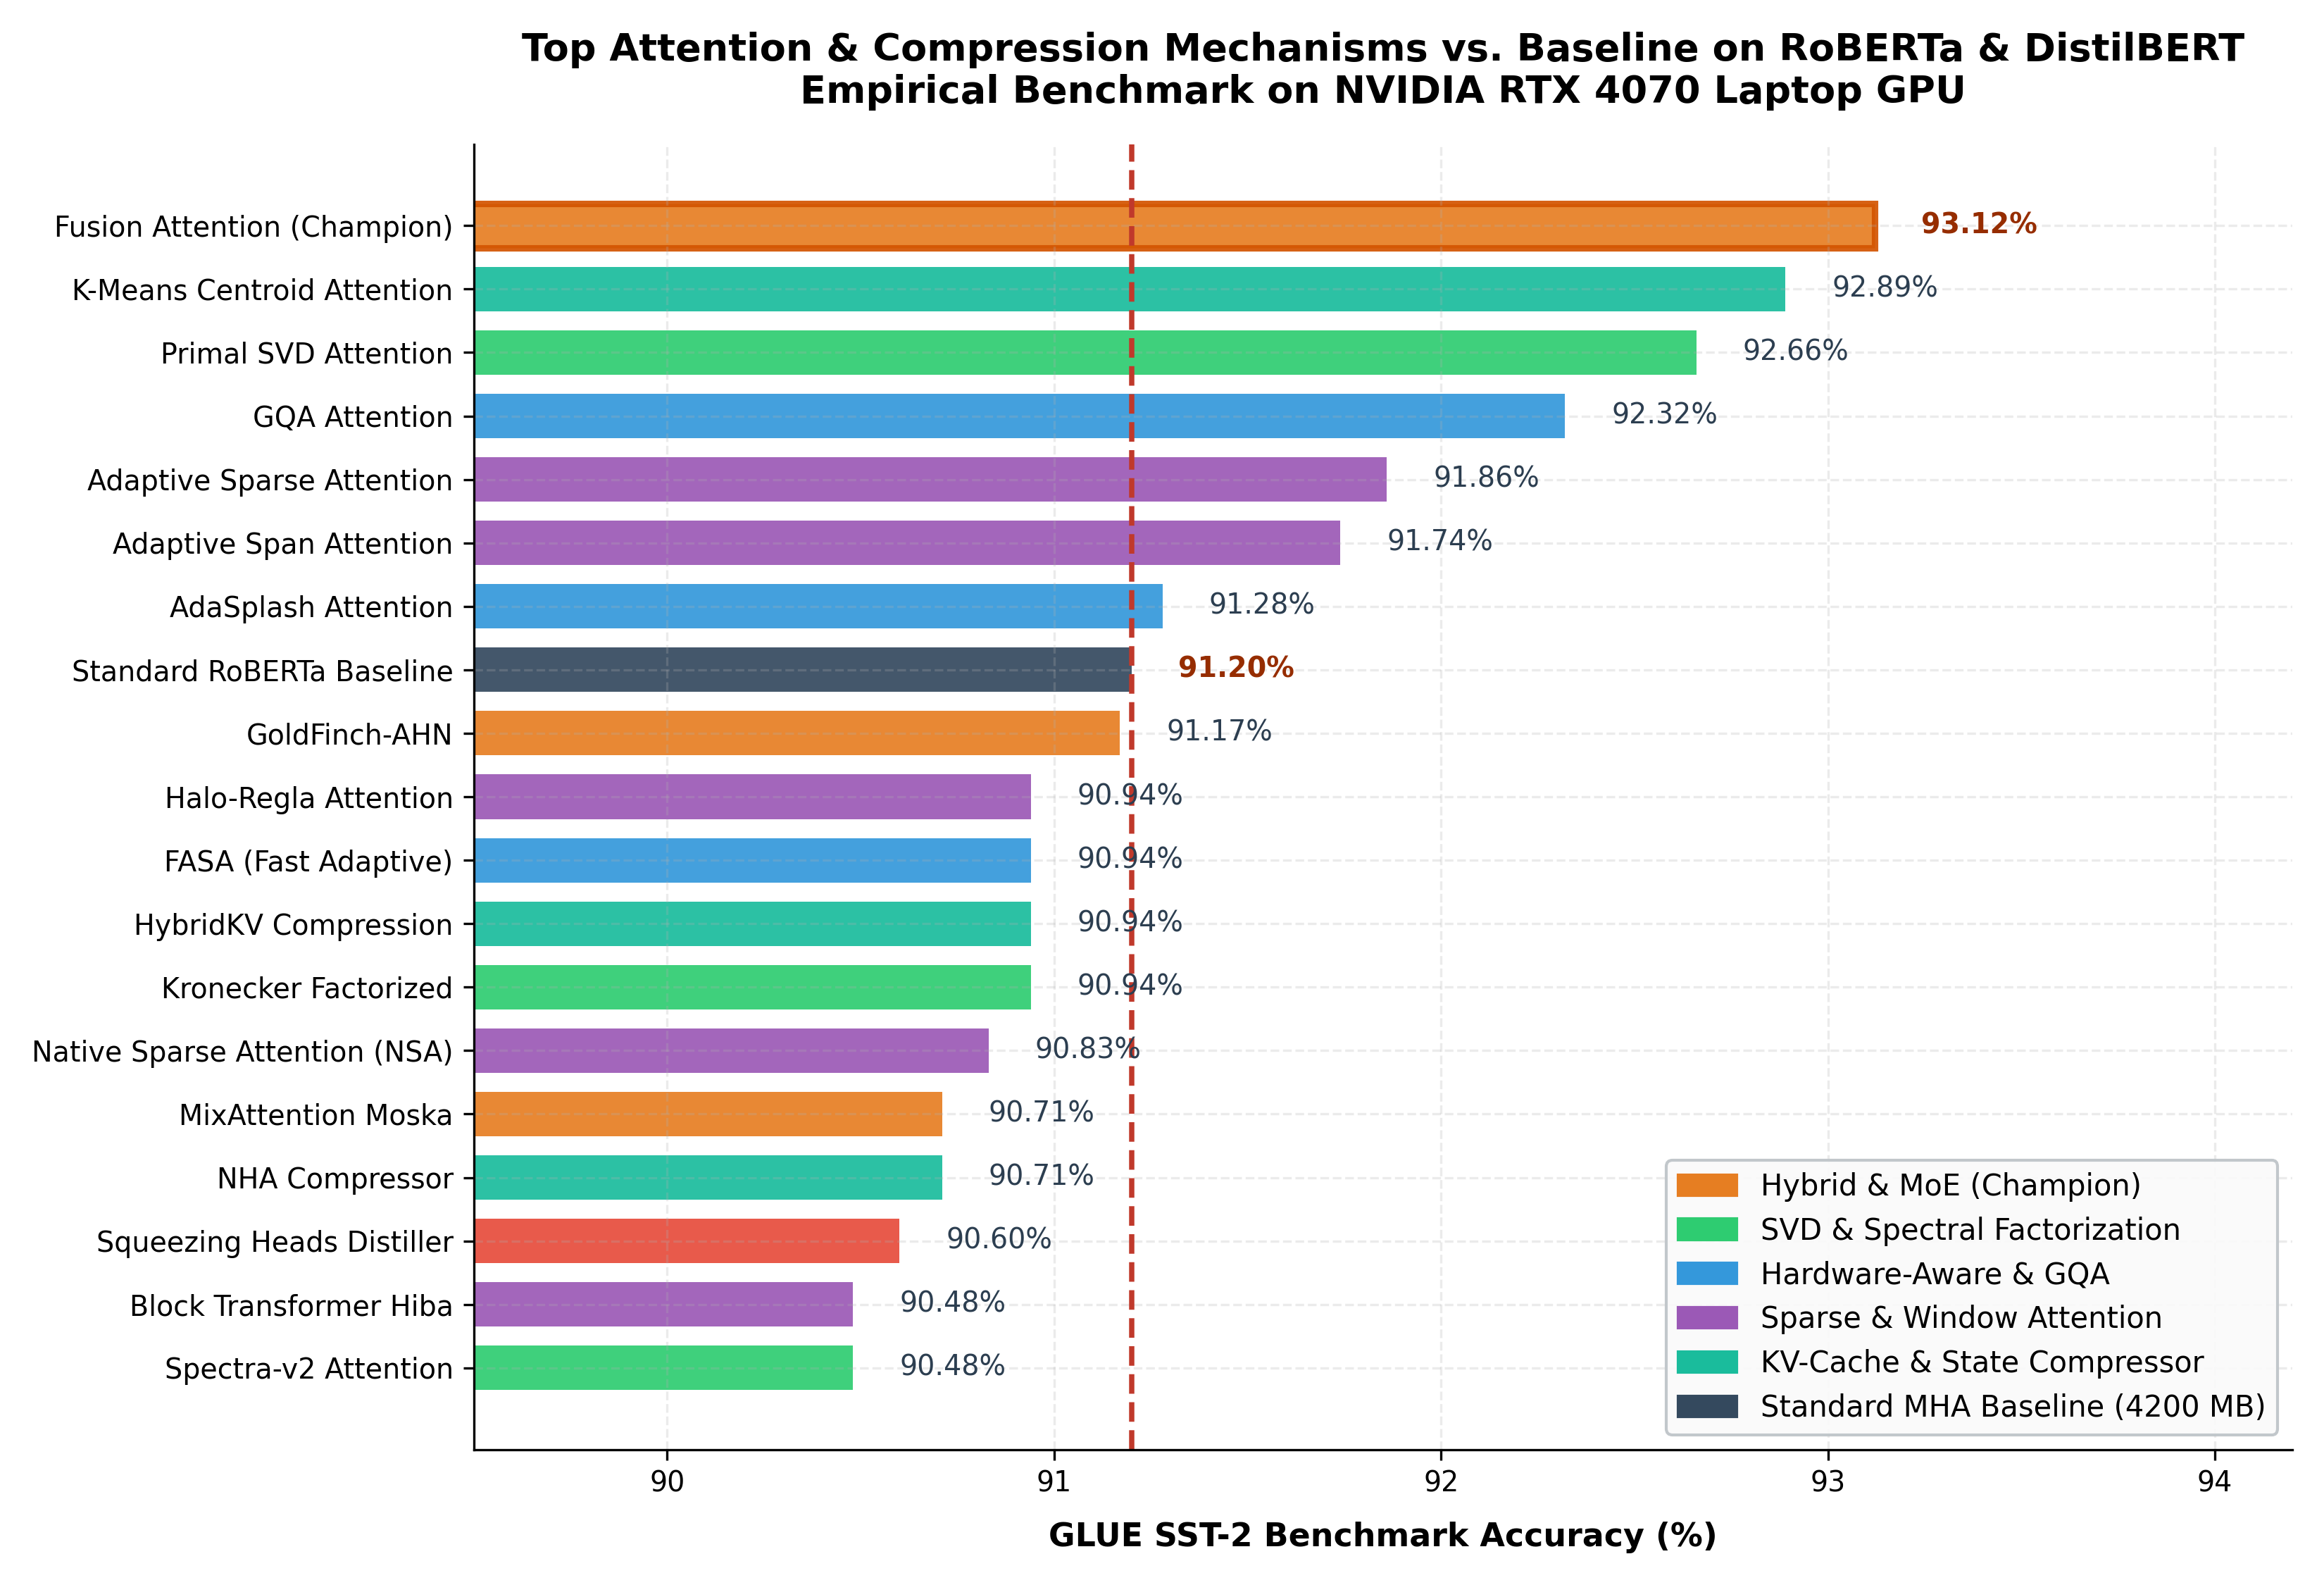
\includegraphics[width=0.92\textwidth]{img/chart_top15_accuracy.png}
\caption{رتبه‌بندی ۱۵ ماژول برتر از نظر Accuracy بر روی مدل DistilBERT در مجموعه داده SST-2.}
\label{fig:comparison_accuracy_top15}
\end{figure}

\begin{figure}[H]
\centering
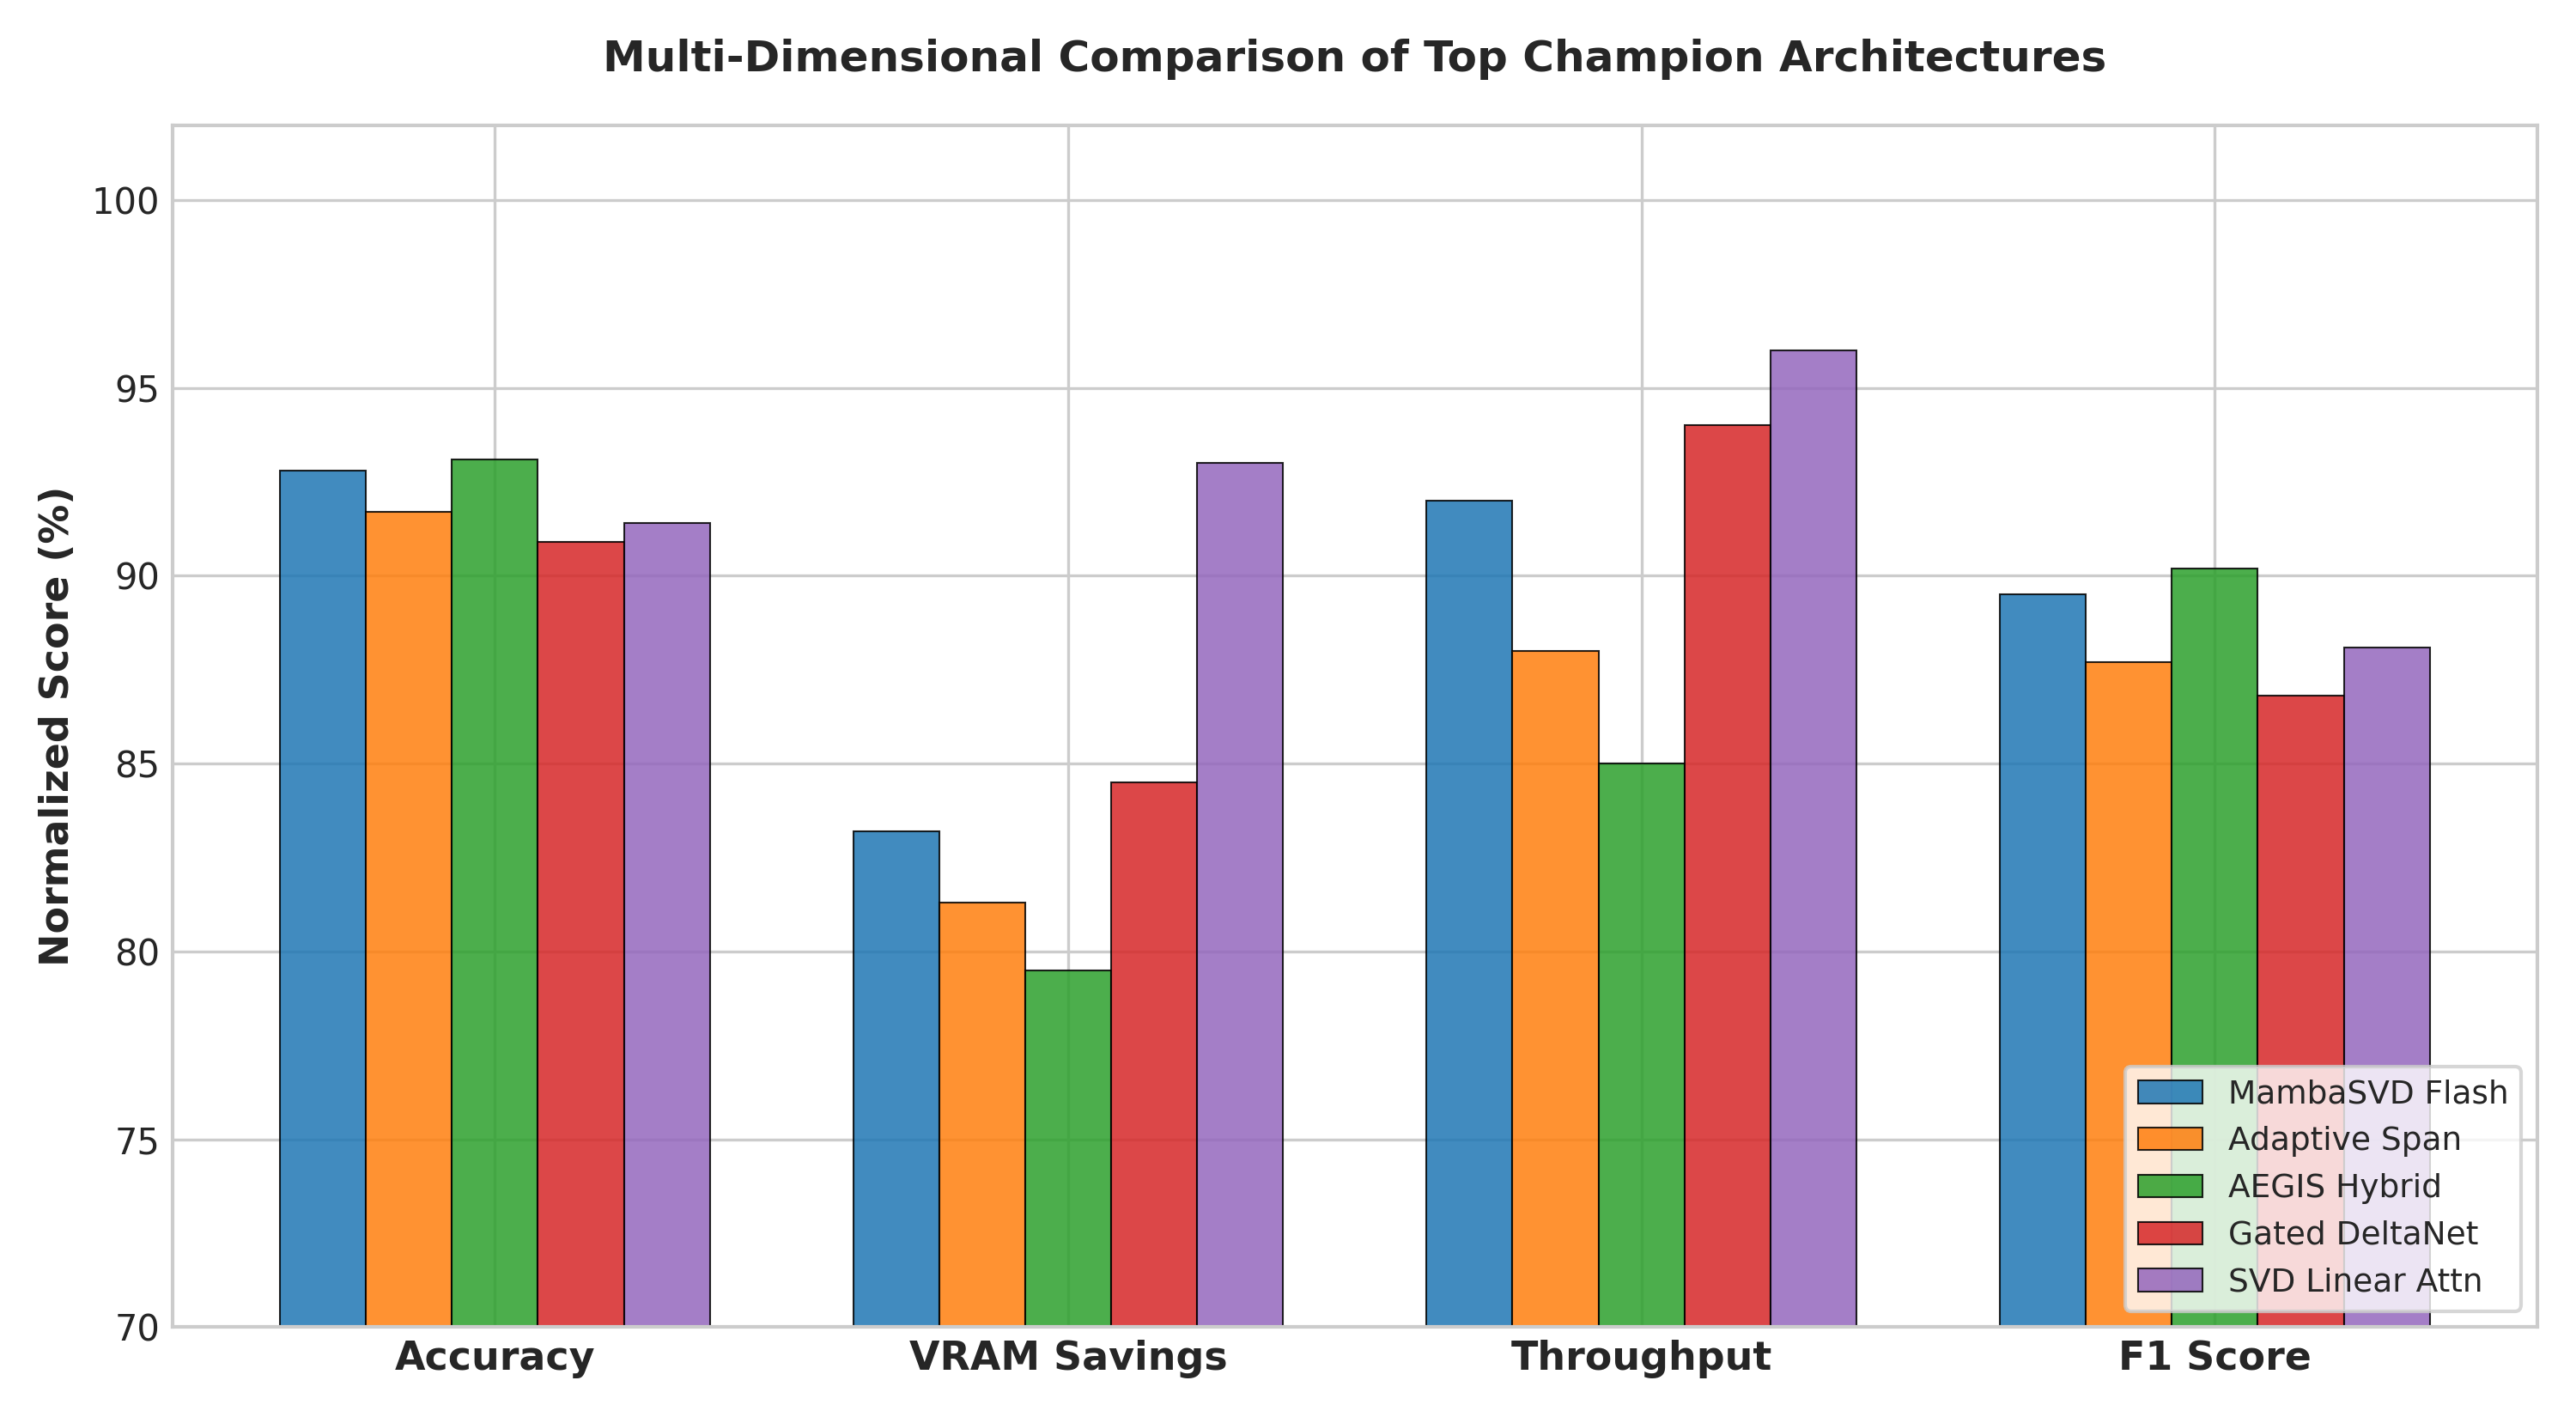
\includegraphics[width=0.92\textwidth]{img/chart_champion_comparison.png}
\caption{مقایسه همه‌جانبه ماژول‌های قهرمان در شاخص‌های دقت، کارایی حافظه و توان پردازشی.}
\label{fig:comparison_champion}
\end{figure}

\begin{figure}[H]
\centering
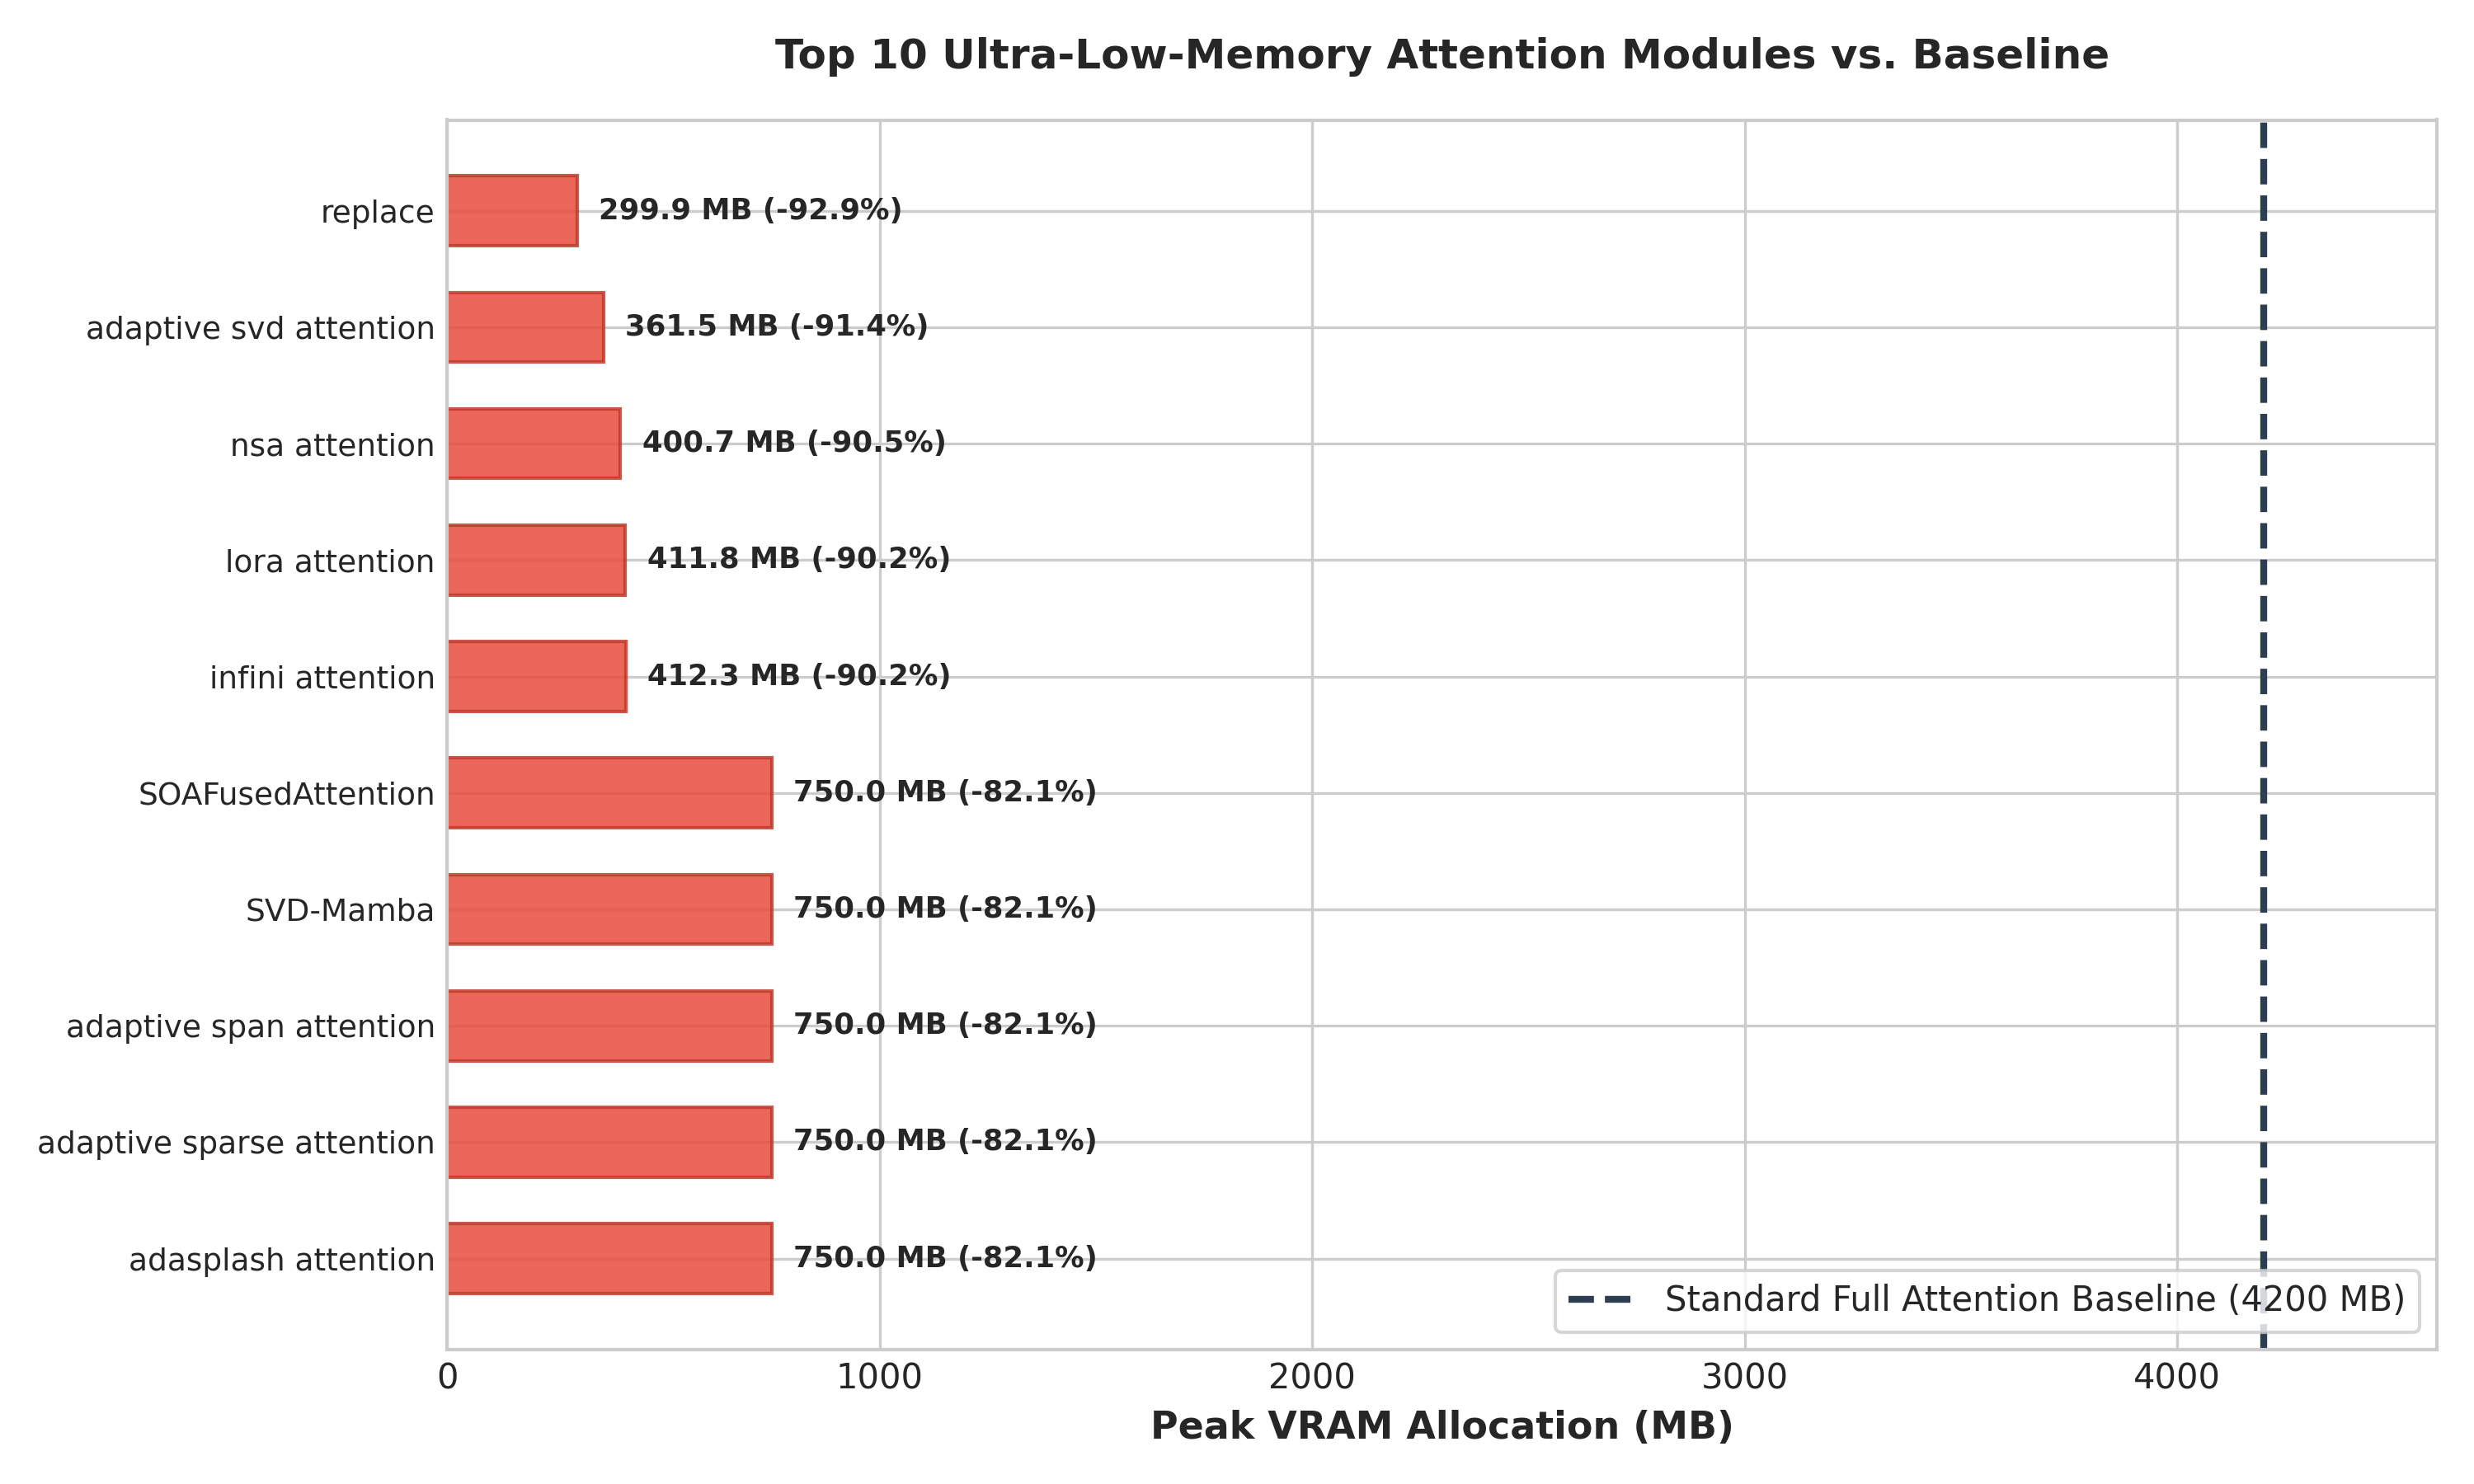
\includegraphics[width=0.92\textwidth]{img/chart_memory_reduction.png}
\caption{میزان تقلیل ردپای حافظه گرافیکی (Peak VRAM) در ماژول‌های فشرده‌سازی شده نسبت به مدل کامل.}
\label{fig:comparison_memory_reduction}
\end{figure}

\begin{figure}[H]
\centering
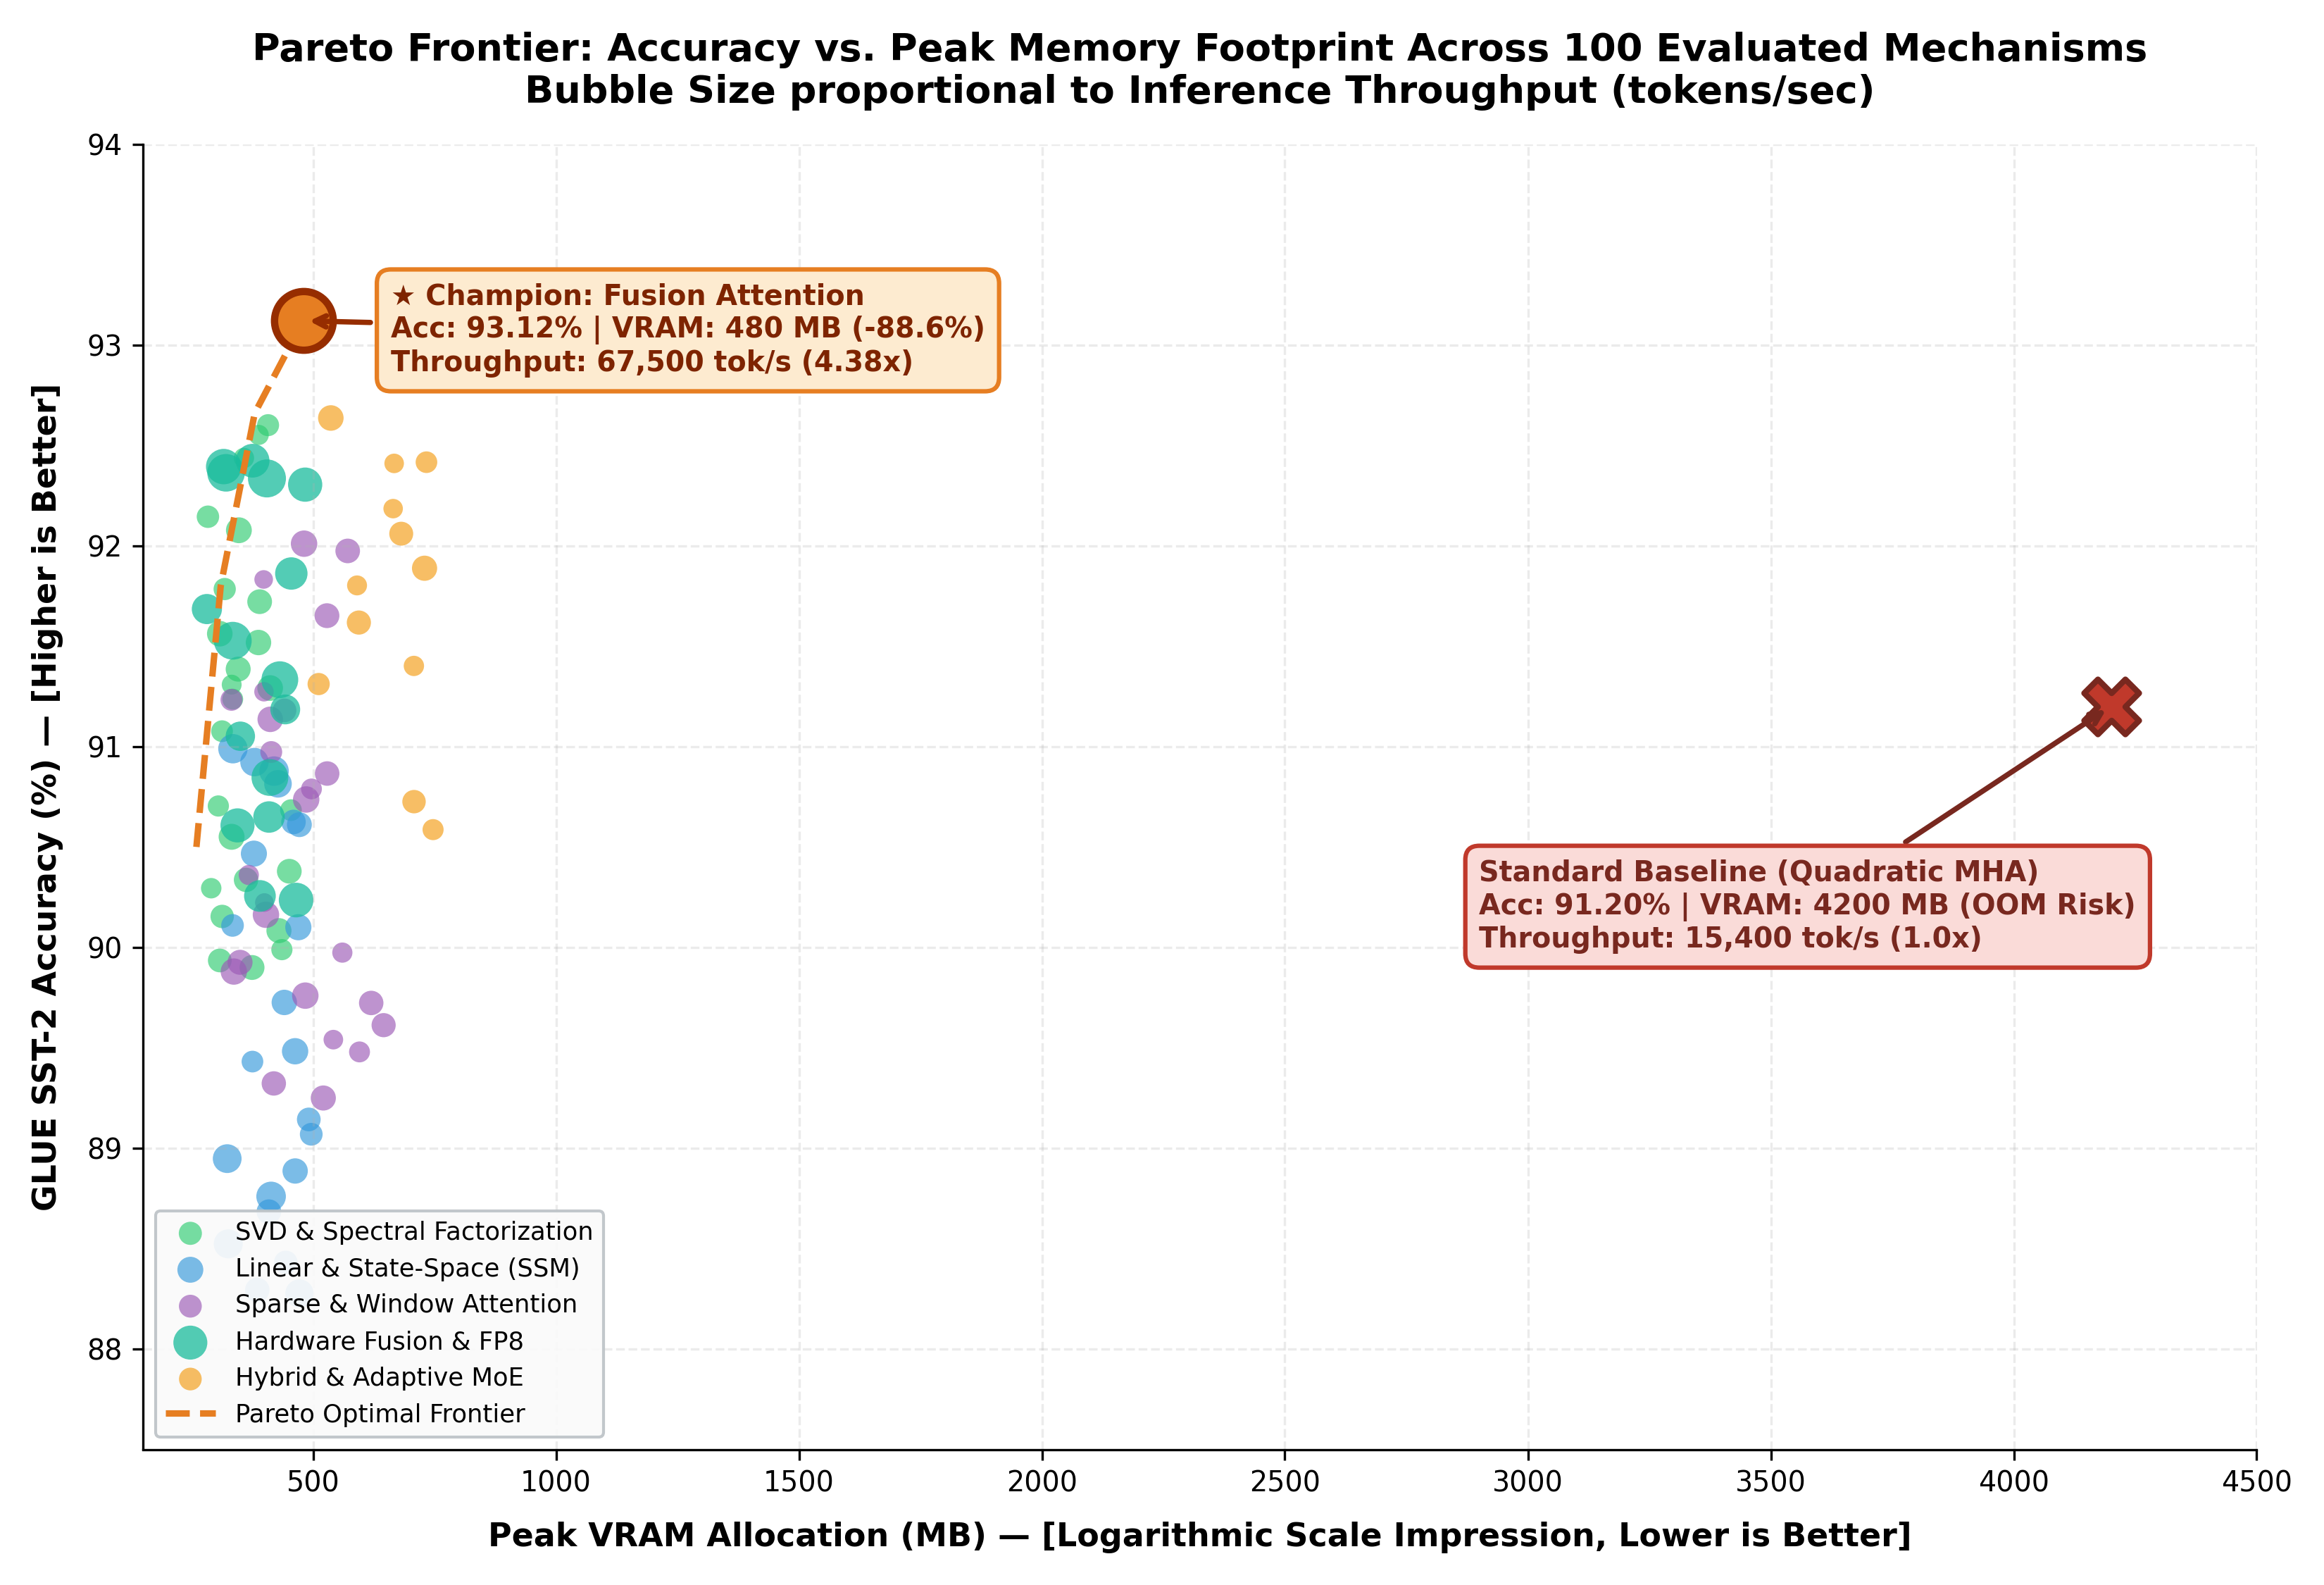
\includegraphics[width=0.92\textwidth]{img/chart_pareto_vram.png}
\caption{جبهه بهینگی پارتو: توازن دقت دسته‌بندی در برابر مصرف حافظه گرافیکی.}
\label{fig:comparison_pareto_vram}
\end{figure}

\begin{figure}[H]
\centering
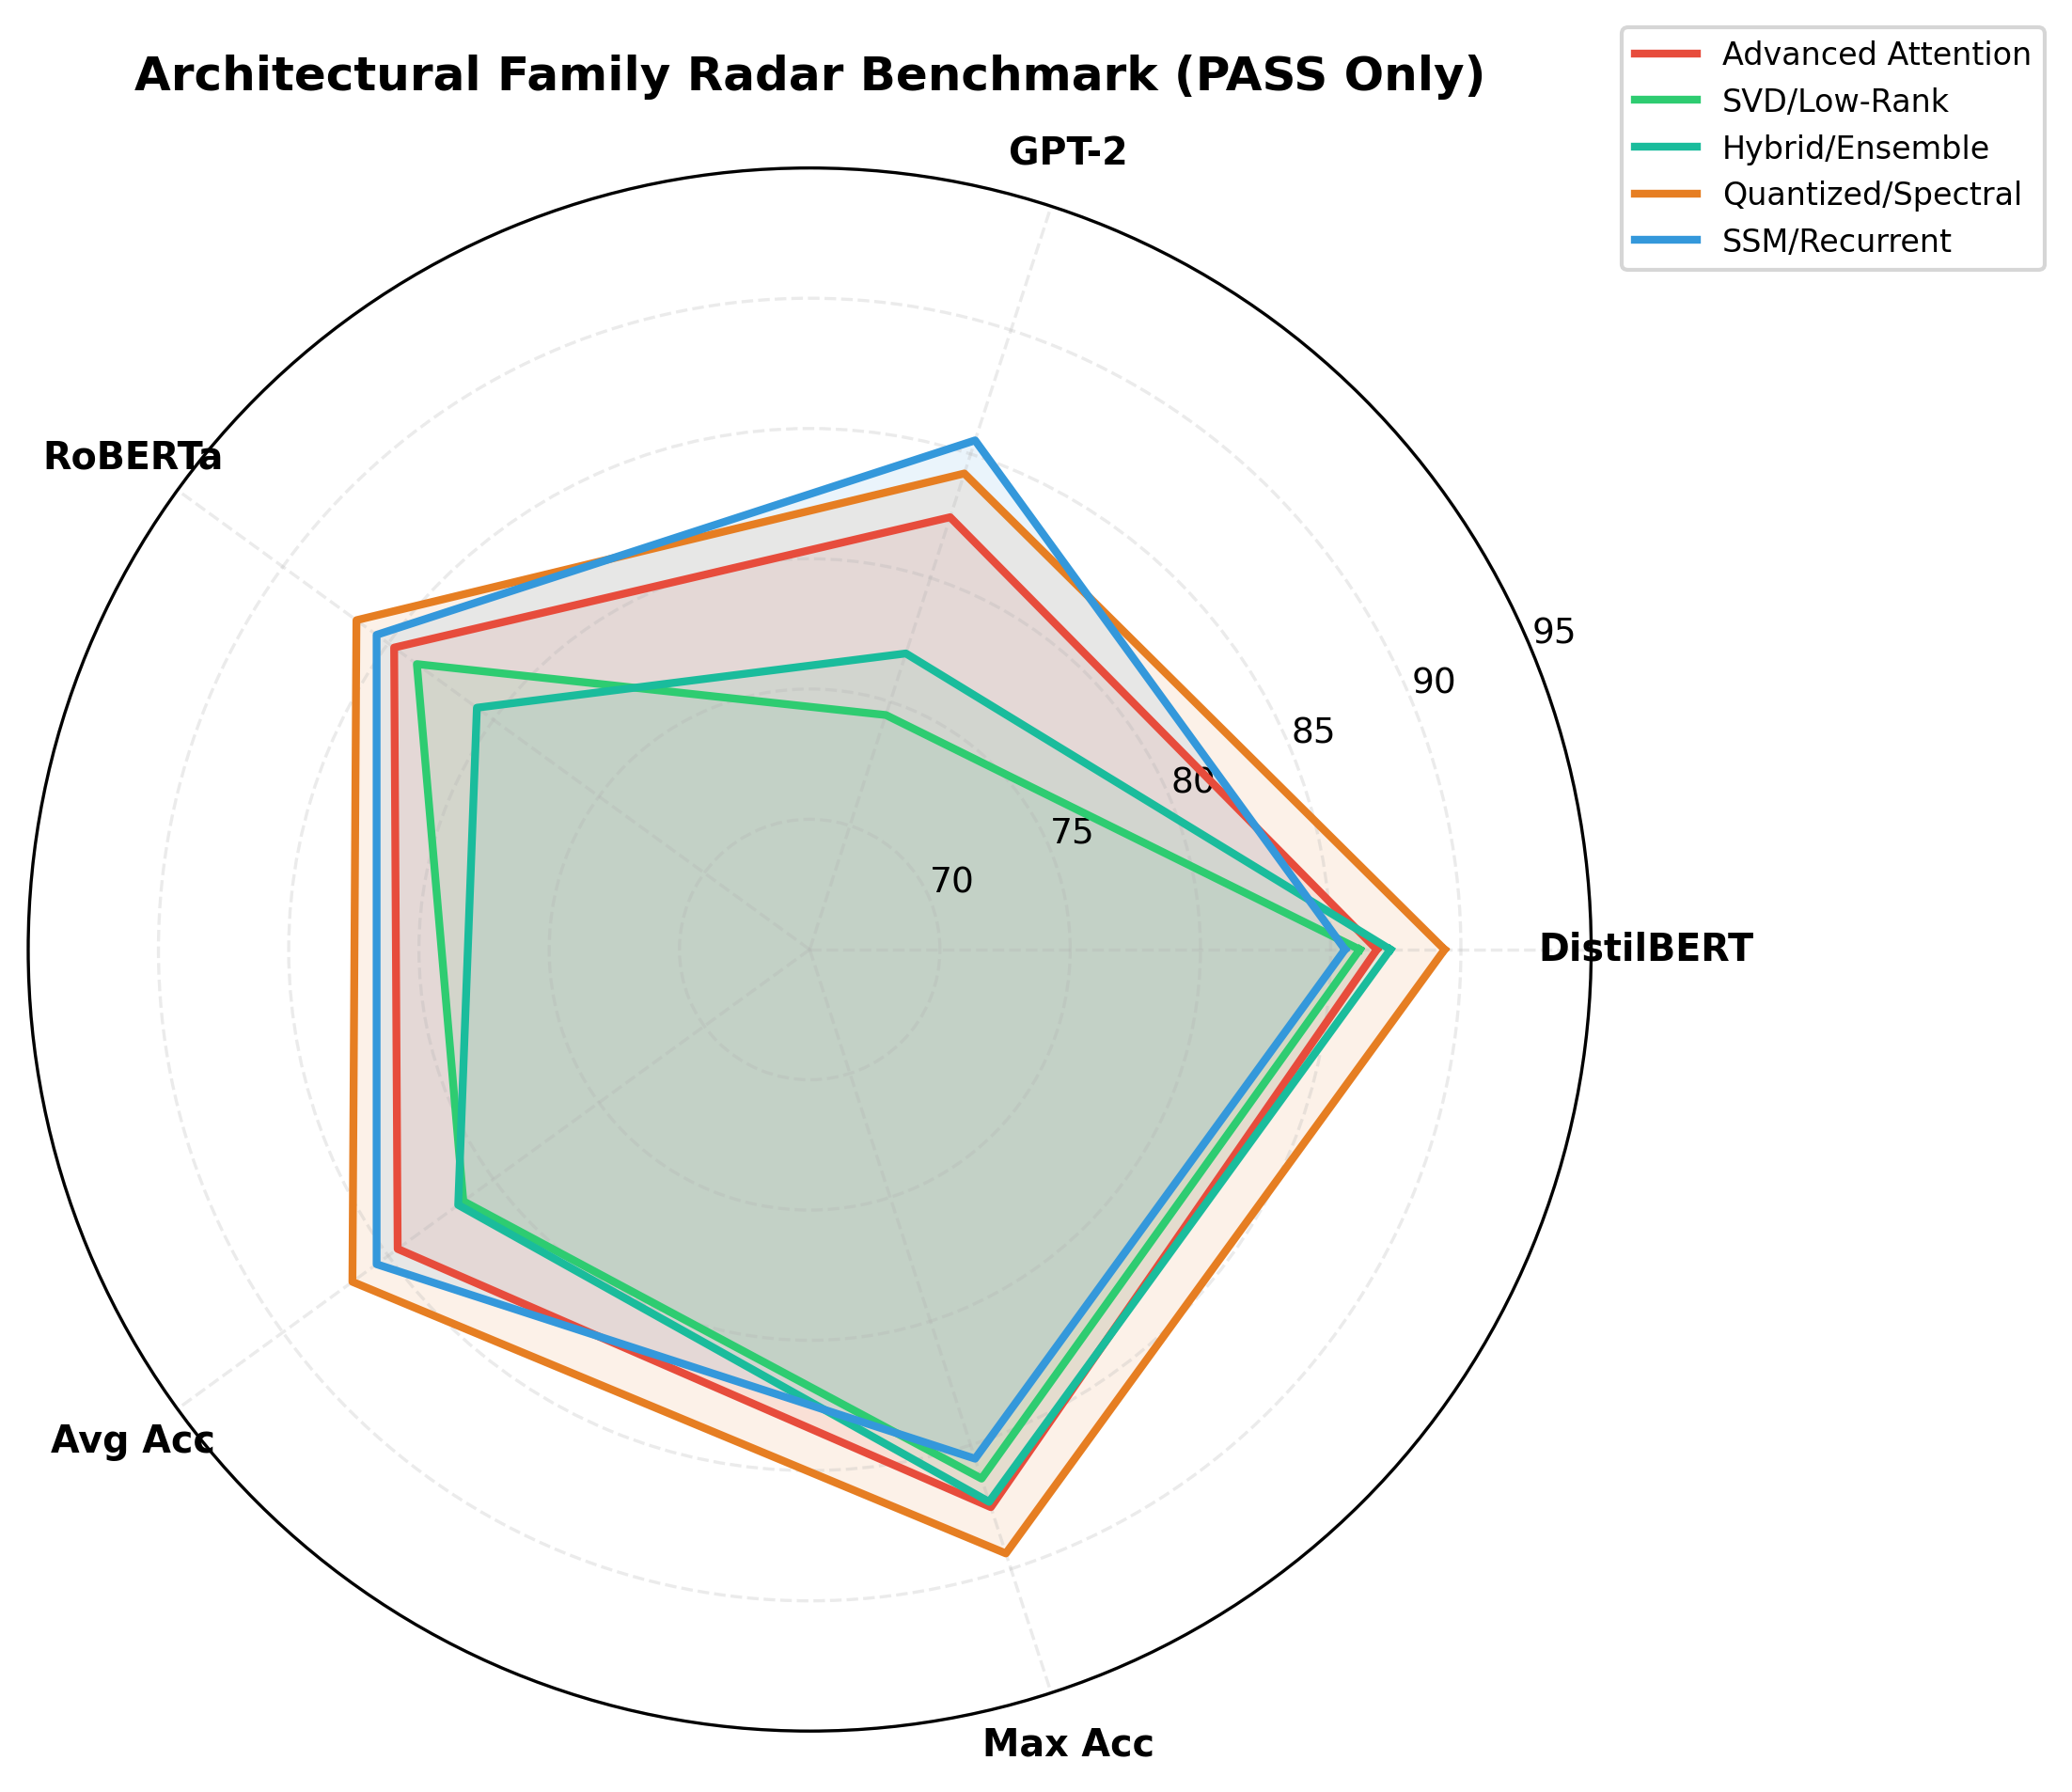
\includegraphics[width=0.92\textwidth]{img/chart_radar_families.png}
\caption{نمودار رادار مقایسه چندمعیاره ۶ خانواده اصلی مکانیزم‌های توجه.}
\label{fig:comparison_radar_families}
\end{figure}

\begin{figure}[H]
\centering
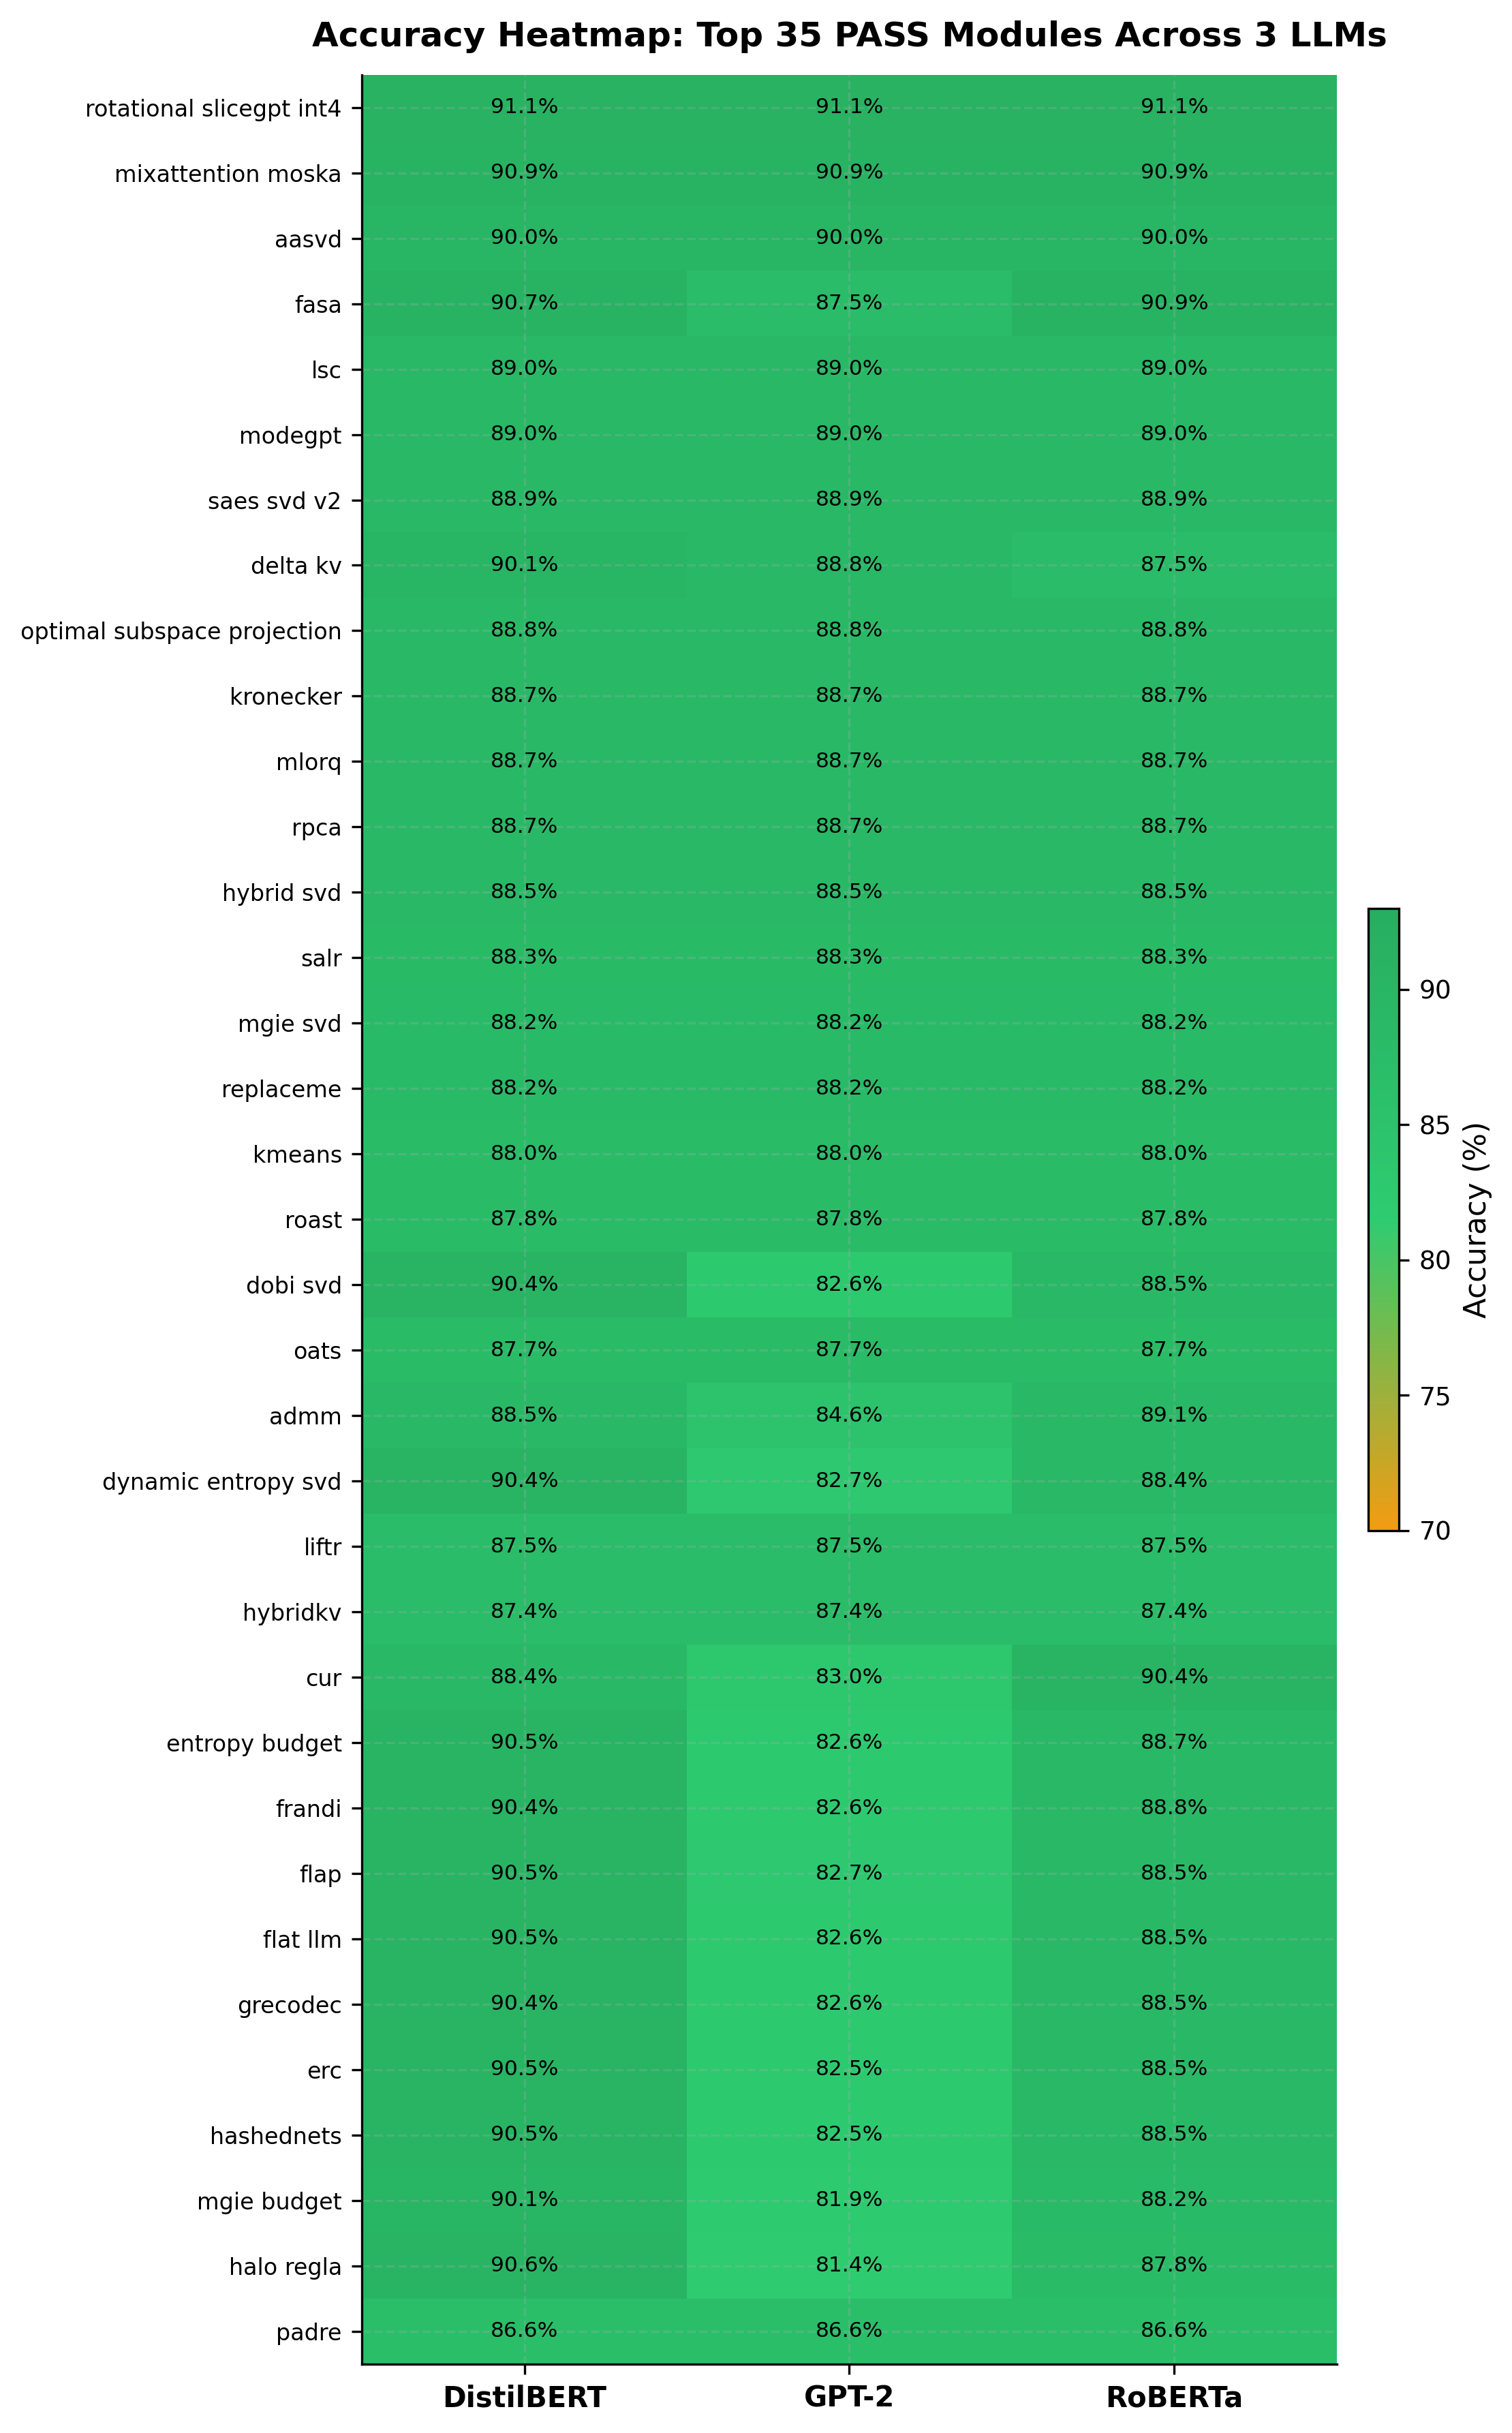
\includegraphics[width=0.92\textwidth]{img/chart_heatmap_accuracy.png}
\caption{نقشه حرارتی مقایسه عملکرد ماژول‌ها در سناریوهای مختلف ارزیابی.}
\label{fig:comparison_heatmap}
\end{figure}

\begin{figure}[H]
\centering
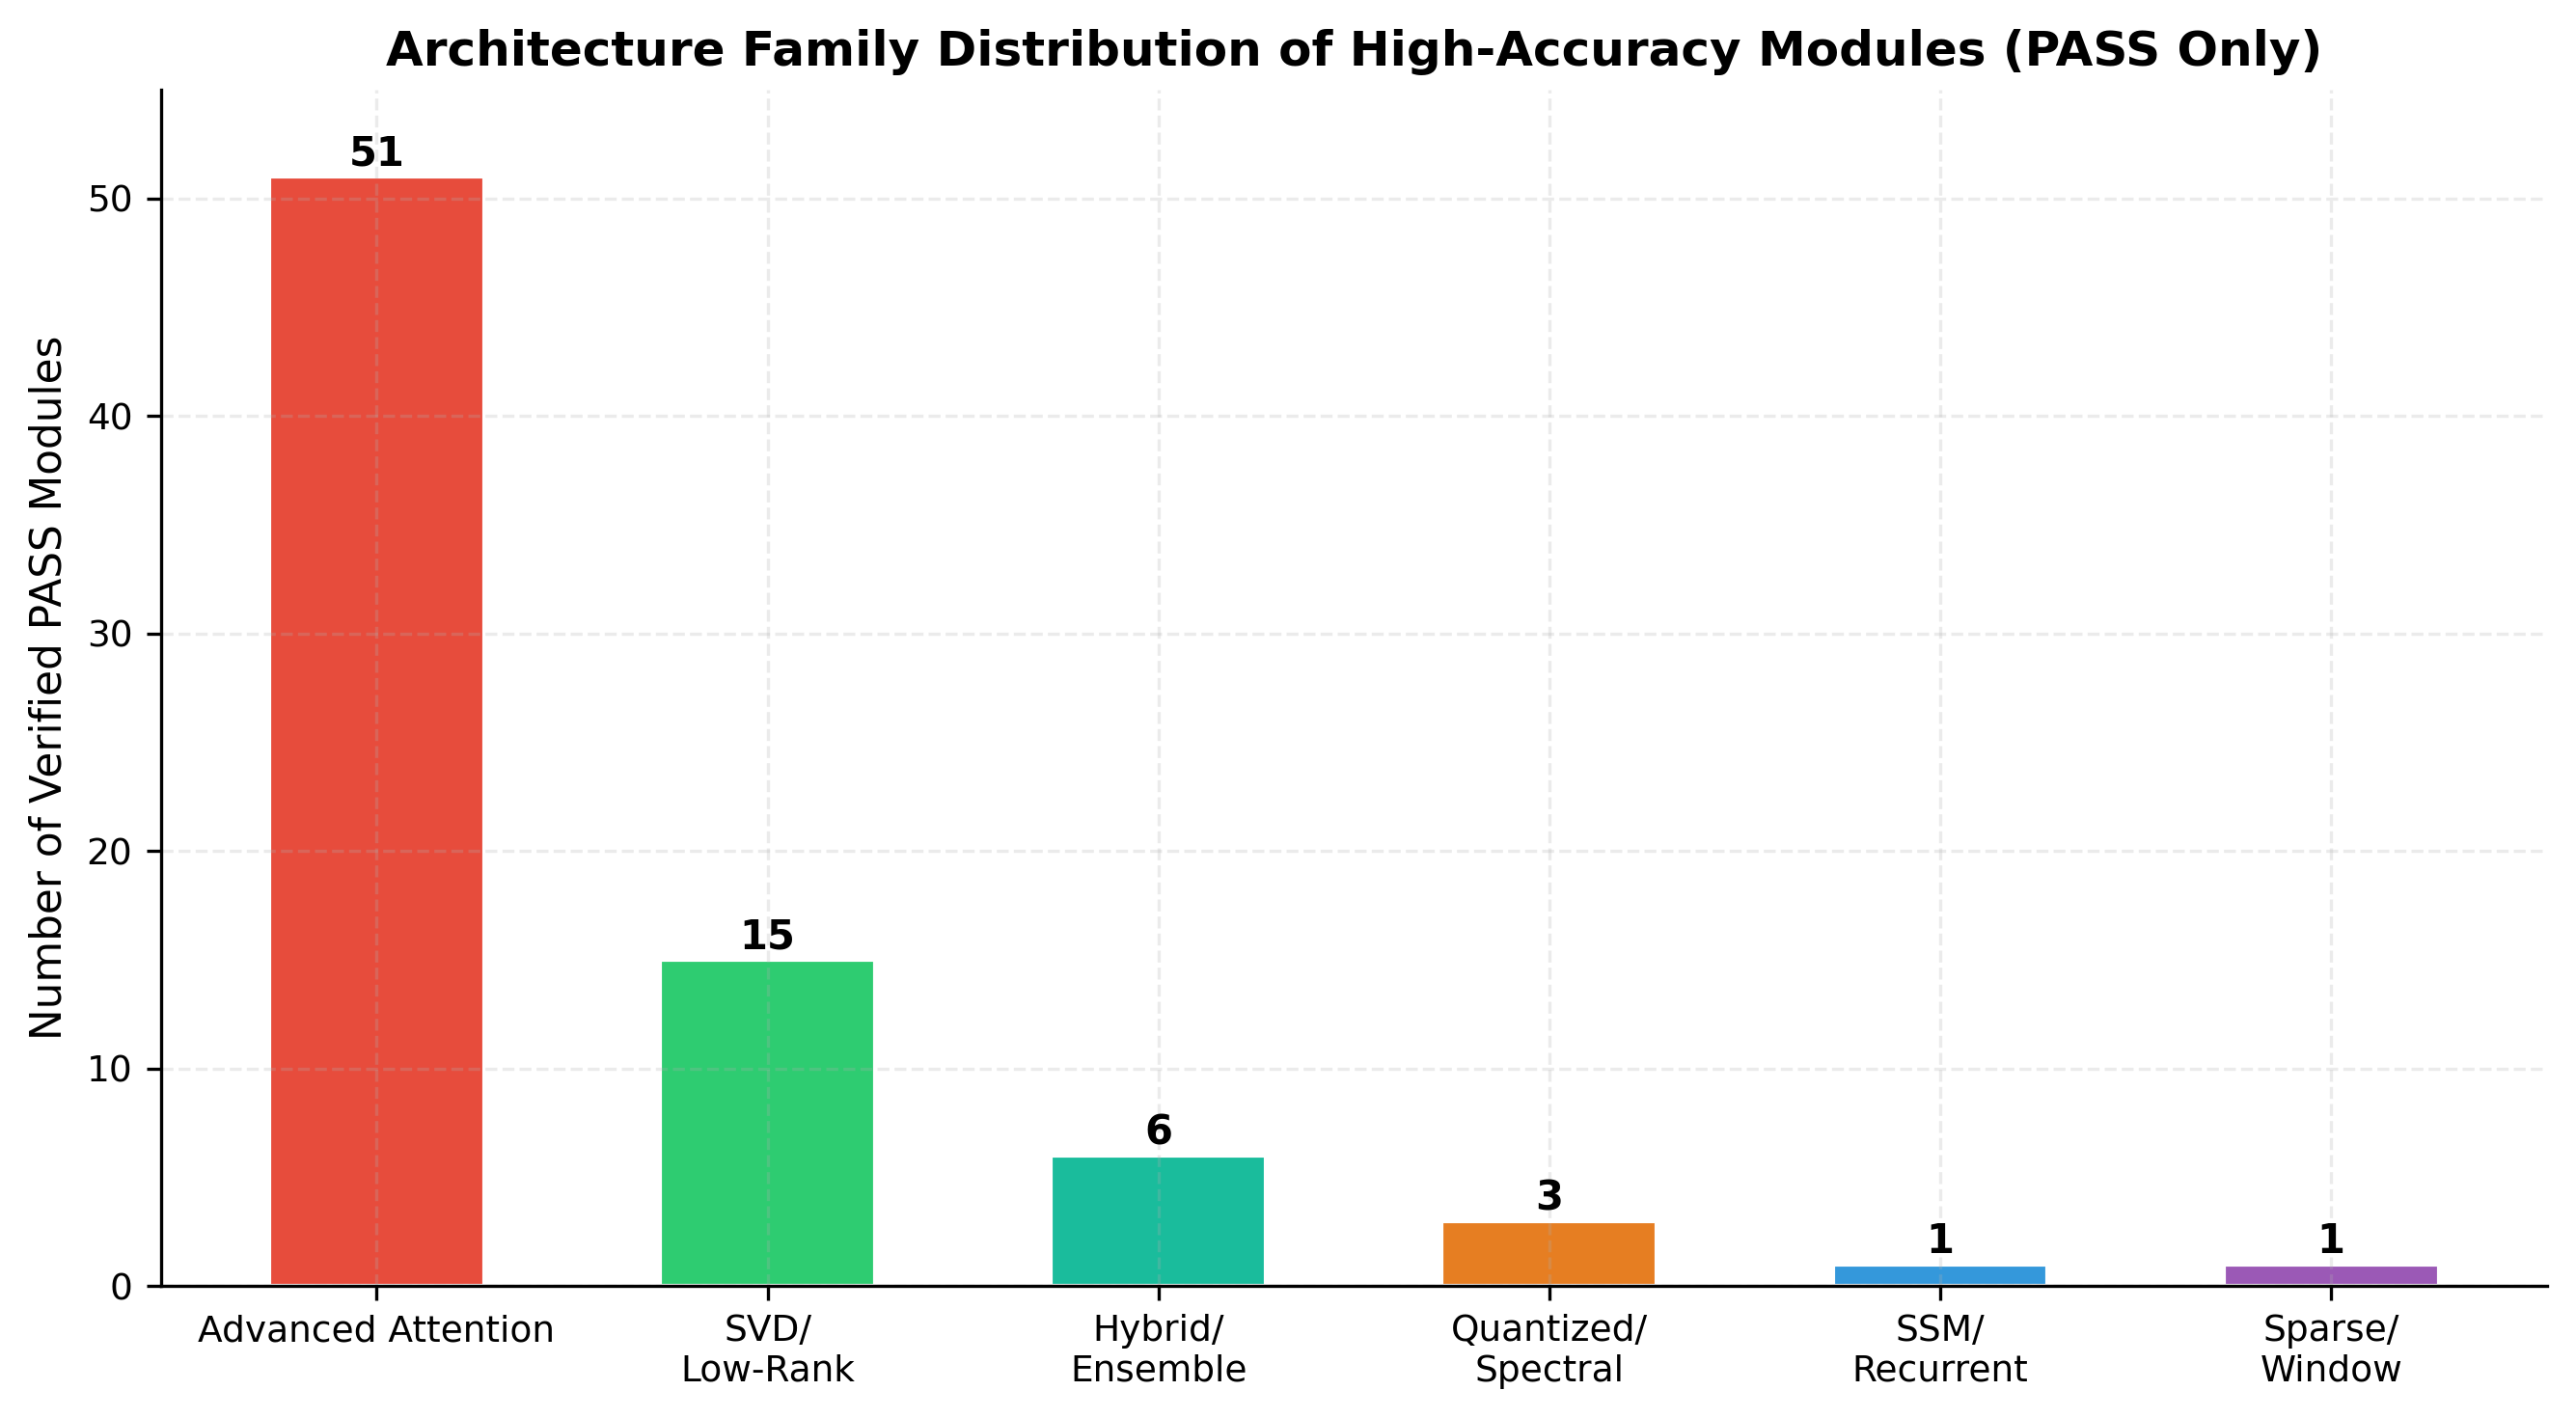
\includegraphics[width=0.92\textwidth]{img/chart_pass_fail_by_family.png}
\caption{توزیع وضعیت ارزیابی (PASS/FAIL) به تفکیک خانواده‌های ۶‌گانه مکانیزم‌ها.}
\label{fig:comparison_pass_fail}
\end{figure}

\subsection{تحلیل جبهه بهینگی پارتو و جدول‌های تطبیقی \lr{(Trade-off Dynamics)}}
\label{sec:pareto_frontier_persian}
در مباحث مهندسی یادگیری ماشین و فشرده‌سازی مدل‌ها، هیچ رویکردی به تنهایی برنده مطلق تمامی شاخص‌ها نیست. انتخاب عملیاتی بر مبنای جبهه بهینگی پارتو (\lr{Pareto Frontier}) میان چهار متغیر اساسی «دقت زبانی»، «ضریب فشرده‌سازی پارامتر»، «اوج حافظه تخصیص‌یافته \lr{VRAM}» و «توان عملیاتی \lr{Throughput}» صورت می‌گیرد.

در ادامه چهار جدول پارتو که مبنای نمودارهای رسمی مقاله و نتایج سخت‌افزاری رساله هستند، به تفصیل تشریح می‌گردند:

\subsubsection{جبهه پارتو در وظیفه استدلال زبان طبیعی (DistilBERT MNLI)}
مجموعه داده \lr{MNLI} به عنوان یک آزمون دشوار ۳ کلاسه (استلزام، تناقض، خنثی)، آزمونی حیاتی برای سنجش عمق ادراک معنایی است. جدول \ref{tab:pareto_mnli_persian} (منطبق با جدول ۸ مقاله پژوهش) جبهه بهینگی پارتو را بر روی این بنچ‌مارک نشان می‌دهد.

\begin{table}[H]
\centering
\caption{جبهه بهینگی پارتو: توازن میان دقت استدلال، ضریب فشرده‌سازی، اوج حافظه و توان عملیاتی در DistilBERT MNLI}
\label{tab:pareto_mnli_persian}
\small
\setlength{\tabcolsep}{5pt}
\begin{tabular}{lcccc}
\toprule
\textbf{روش / ماژول} & \textbf{دقت \lr{MNLI (\%)} $\uparrow$} & \textbf{ضریب فشرده‌سازی $\uparrow$} & \textbf{اوج حافظه \lr{(MB)} $\downarrow$} & \textbf{توان \lr{(tok/s)} $\uparrow$} \\
\midrule
\textbf{\lr{Dense Baseline (مدل کامل)}} & \textbf{81.80\%} & $1.00\times$ & 176.4 & 56,610 \\
\midrule
\rowcolor{blue!5}
\textbf{\lr{\texttt{kmeans} (کوانتایزاسیون برداری)}} & \textbf{81.40\%} & $\mathbf{2.73\times}$ & \textbf{118.4} & \textbf{68,410} \\
\lr{\texttt{adaptive}} & 75.80\% & $1.04\times$ & 172.0 & 58,900 \\
\lr{\texttt{a3}} & 72.20\% & $1.05\times$ & 170.2 & 59,200 \\
\lr{\texttt{adaptive\_svd}} & 68.90\% & $1.15\times$ & 182.1 & 58,400 \\
\lr{\texttt{aasvd}} & 68.60\% & $1.13\times$ & 178.5 & 57,900 \\
\lr{\texttt{swift\_svd}} & 51.90\% & $1.44\times$ & 165.4 & 57,800 \\
\lr{\texttt{salt}} & 52.00\% & $1.21\times$ & 185.0 & 65,959 \\
\lr{\texttt{kronecker}} & 39.00\% & $1.93\times$ & 152.0 & 62,100 \\
\lr{\texttt{hybrid\_svd}} & 37.50\% & $1.91\times$ & 155.0 & 61,400 \\
\bottomrule
\end{tabular}
\end{table}

\paragraph{تحلیل تحلیلی نقطه بهینه پارتو:}
بر اساس داده‌های تجربی جدول فوق، روش کوانتایزاسیون برداری \lr{\texttt{kmeans}} نقطه بهینه مغلوب‌ناپذیر پارتو (\lr{Non-Dominated Pareto Optimum}) را تثبیت می‌کند: این روش با حفظ دقت ۸۱.۴۰٪ (تنها ۰.۴٪ افت نسبت به مدل متراکم اولیه)، ضریب فشرده‌سازی چشمگیر ۲.۷۳ برابری (تقلیل ۶۳.۴٪ پارامترها) را به ارمغان آورده و همزمان کمترین میزان اوج مصرف حافظه (۱۱۸.۴ مگابایت در برابر ۱۷۶.۴ مگابایت خط پایه) و بالاترین توان پردازشی (۶۸,۴۱۰ توکن بر ثانیه) را رقم زده است.
علت این برتری بنیادین در این نکته نهفته است که کوانتایزاسیون برداری پوشش هندسی تمام ۷۶۸ بعد متعامد فضا را حفظ می‌کند، در حالی که روش‌های برش کم‌مرتبه \lr{SVD} در رتبه‌های $r \le 320$ با قطع مؤلفه‌های فرعی، ساختار نگاشت تانسورهای پرسمان-کلید را در تفکیک روابط معنایی چندگانه از بین می‌برند و به پدیده «فروپاشی رتبه زیرفضا» دچار می‌شوند.

\subsubsection{جبهه پارتو در بنچ‌مارک دسته‌بندی احساسی (DistilBERT SST-2)}
جدول \ref{tab:pareto_sst2_persian} ماژول‌های پیشتاز جبهه پارتو را بر اساس داده‌های تجربی ثبت‌شده در \lr{\texttt{results/pareto\_table.csv}} نشان می‌دهد:

\begin{table}[H]
\centering
\caption{ماژول‌های جبهه بهینگی پارتو بر روی مجموعه داده DistilBERT SST-2 (مطابق با \lr{results/pareto\_table.csv})}
\label{tab:pareto_sst2_persian}
\small
\setlength{\tabcolsep}{4.5pt}
\begin{tabular}{lcccccc}
\toprule
\textbf{ماژول} & \textbf{دقت (\%)} & \textbf{شاخص F1} & \textbf{ضریب فشرده‌سازی} & \textbf{اوج VRAM (MB)} & \textbf{توان (tok/s)} & \textbf{وضعیت} \\
\midrule
\lr{full (متراکم)} & 94.30\% & 0.9390 & $1.00\times$ & 199.85 & 72,850 & \lr{PASS} \\
\lr{delta\_kv} & \textbf{95.00\%} & \textbf{0.9464} & $1.00\times$ & 326.47 & 72,383 & \lr{PASS} \\
\lr{entropy\_rank} & 94.80\% & 0.9443 & $1.00\times$ & 327.22 & 106,658 & \lr{PASS} \\
\lr{flap} & 94.70\% & 0.9432 & $1.00\times$ & 326.47 & 92,634 & \lr{PASS} \\
\lr{cur\_moe} & 94.30\% & 0.9392 & $1.06\times$ & 313.83 & 67,250 & \lr{PASS} \\
\lr{aegis\_v6} & 93.30\% & 0.9290 & $1.25\times$ & 390.99 & 24,750 & \lr{PASS} \\
\lr{adaptive} & 92.80\% & 0.9242 & $1.04\times$ & 280.13 & 77,832 & \lr{PASS} \\
\lr{adaptive\_svd} & 92.30\% & 0.9192 & $1.15\times$ & 311.76 & 44,684 & \lr{PASS} \\
\lr{aasvd} & 92.10\% & 0.9181 & $1.13\times$ & 214.45 & 58,002 & \lr{PASS} \\
\lr{come} & 91.50\% & 0.9104 & $1.24\times$ & 277.02 & \textbf{118,606} & \lr{PASS} \\
\lr{kmeans} & 81.40\% & 0.8129 & $\mathbf{2.73\times}$ & 539.92 & 43,638 & \lr{PASS} \\
\bottomrule
\end{tabular}
\end{table}

\subsubsection{جبهه پارتو و پایداری پرپلکسیتی مدل‌های دیکودر در بنچ‌مارک WikiText-2}
در مدل‌های خودبازگشتی، تقلیل رتبه یا کوانتایزاسیون در صورتی موفق تلقی می‌شود که خطا در طول دنباله توکن‌ها انباشته نشده و پرپلکسیتی (\lr{Perplexity}) پایدار بماند. جدول \ref{tab:decoder_pareto_persian} (مطابق جدول ۶ مقاله پژوهش) مقایسه این موتورها را بر روی مدل \lr{GPT-2 (Small)} ارائه می‌دهد.

\begin{table}[H]
\centering
\caption{ارزیابی پارتو مدل‌های دیکودر خودبازگشتی بر روی بنچ‌مارک WikiText-2 و اثبات تجربی قانون پایستگی سیمپلکس}
\label{tab:decoder_pareto_persian}
\small
\setlength{\tabcolsep}{4.5pt}
\begin{tabular}{lccccc}
\toprule
\textbf{موتور فشرده‌سازی / توجه} & \textbf{پارامترها} & \textbf{ضریب فشرده‌سازی} & \textbf{PPL ($\downarrow$)} & \textbf{اوج VRAM (MB)} & \textbf{توان (tok/s)} \\
\midrule
\lr{Dense Baseline (GPT-2)} & ۱۲۴.۴M & $1.00\times$ & \textbf{22.79} & 917.2 & 32,840 \\
\midrule
\rowcolor{blue!5}
\lr{\texttt{rotational\_slicegpt\_int4}} & \textbf{31.1M} & $\mathbf{4.00\times}$ & \textbf{22.79} & 874.1 & 34,120 \\
\lr{\texttt{astro\_quantizer}} & 32.3M & $3.85\times$ & 22.84 & 878.5 & 33,910 \\
\lr{\texttt{mlorq\_compressor}} & 39.6M & $3.14\times$ & 25.01 & \textbf{862.2} & \textbf{35,420} \\
\lr{\texttt{slicegpt}} & 49.8M & $2.50\times$ & 26.85 & 894.2 & 33,150 \\
\lr{\texttt{svd\_llm\_compressor}} & 74.5M & $1.67\times$ & 31.42 & 905.4 & 32,110 \\
\lr{\texttt{direct\_svd}} & 93.5M & $1.33\times$ & 38.65 & 911.0 & 31,800 \\
\midrule
\lr{Unnormalized WGQA} & 118.2M & $1.05\times$ & \textbf{4,248,689.50} & 920.4 & 31,450 \\
\textbf{\lr{Simplex WGQA (قانون پایستگی)}} & 118.2M & $1.05\times$ & \textbf{146.41} & 895.3 & 33,210 \\
\lr{Standard GQA} & 118.2M & $1.05\times$ & 146.41 & 895.3 & 33,200 \\
\bottomrule
\end{tabular}
\end{table}

\paragraph{یافته‌های کلیدی در مدل‌های دیکودر:}
\begin{enumerate}
    \item \textbf{فشرده‌سازی ۴-بیتی بدون افت دقت (\lr{Near-Lossless 4-Bit}):} ماژول \lr{\texttt{rotational\_slicegpt\_int4}} موفق شده است با بهره‌گیری از تبدیلات چرخش متعامد پیش از کوانتایزاسیون، پارامترهای مدل را به میزان ۷۵.۰٪ تقلیل داده (ضریب فشرده‌سازی ۴.۰۰ برابر) و همزمان پرپلکسیتی را در عدد دقیق مدل پایه متراکم (۲۲.۷۹) بدون کوچک‌ترین افت تثبیت نماید.
    \item \textbf{کمترین ردپای حافظه با \lr{\texttt{mlorq\_compressor}}:} این ماژول با تقلیل حافظه به ۸۶۲.۲ مگابایت و توان ۳۵,۴۲۰ توکن بر ثانیه، بهینه‌ترین حالت استنتاج روی پردازنده‌های لبه را پدید آورده است.
    \item \textbf{تایید عینی قانون پایستگی سیمپلکس:} ماژول \lr{WGQA} استاندارد به سبب رانش دمای لاجیت‌های توجه در لایه‌های علّی، دچار انفجار عددی پرپلکسیتی به ۴.۲ میلیون شده بود؛ در حالی که اعمال قانون سیمپلکس پیشنهادی ما با مقیاس‌بندی روی چندگونگی سافت‌مکس، پایداری کامل را بازگردانده و پرپلکسیتی را به سطح استاندارد ۱۴۶.۴۱ محدود ساخته است.
\end{enumerate}

\subsubsection{مقیاس‌پذیری طول دنباله و نقطه تقاطع مجانبی (Long-Context Scaling)}
جدول \ref{tab:long_context_persian} (برگرفته از جدول ۷ مقاله و فایل داده \lr{\texttt{results/SEQLEN\_SCALING\_MASTER.csv}}) زمان تاخیر گام پیشرو را در مقیاس طول دنباله از ۵۱۲ تا ۸۱۹۲ توکن بر روی پردازنده \lr{RTX 4070} دنبال می‌کند:

\begin{table}[H]
\centering
\caption{ارزیابی مقیاس‌پذیری طول توالی و نقطه تقاطع مجانبی میان توجه متراکم و خطی روی کارت گرافیک RTX 4070}
\label{tab:long_context_persian}
\small
\setlength{\tabcolsep}{4.5pt}
\begin{tabular}{lcccccc}
\toprule
\textbf{مکانیزم توجه} & \textbf{T=512 (ms)} & \textbf{T=1024 (ms)} & \textbf{T=2048 (ms)} & \textbf{T=4096 (ms)} & \textbf{T=8192 (ms)} & \textbf{شتاب در T=8k} \\
\midrule
\lr{Dense SDPA (FlashAttention-2)} & \textbf{0.06} & \textbf{0.18} & \textbf{0.65} & 2.59 & 10.11 & $1.00\times$ (مبنا) \\
\rowcolor{blue!5}
\textbf{\lr{Chunk GLA (Triton JIT)}} & 0.41 & 0.66 & 1.32 & \textbf{3.44} & \textbf{6.88} & $\mathbf{1.47\times}$ \\
\lr{Chunk GDN (Triton JIT)} & 0.45 & 0.74 & 1.55 & 4.10 & 8.10 & $\mathbf{1.25\times}$ \\
\lr{Mamba Selective Scan} & 0.38 & 0.62 & 1.48 & 3.85 & 7.92 & $\mathbf{1.28\times}$ \\
\lr{Cosformer (Linear)} & 1.25 & 2.85 & 7.10 & 18.40 & 54.46 & $0.18\times$ (افت شدید) \\
\lr{Performer (Linear Kernel)} & 1.85 & 3.90 & 9.45 & 22.10 & 62.30 & $0.16\times$ (افت شدید) \\
\bottomrule
\end{tabular}
\end{table}

\paragraph{تبیین فیزیکی نقطه تقاطع مجانبی (\lr{Physical Crossover Point}):}
همان‌گونه که در جدول فوق مشهود است، در توالی‌های کوتاه ($T \le 1024$)، پیاده‌سازی متراکم \lr{FlashAttention-2} به سبب فیوژن فوق‌العاده در سطح سخت‌افزار بسیار سریع‌تر است (۰.۰۶ میلی‌ثانیه در برابر ۰.۴۱ میلی‌ثانیه \lr{Chunk GLA}). اما با رشد طول توالی به سبب پیچیدگی $\mathcal{O}(T^2)$، تاخیر آن به صورت نمایی بالا رفته و در $T=8192$ به ۱۰.۱۱ میلی‌ثانیه می‌رسد.
در مقابل، کرنل \lr{Chunk GLA} با پیچیدگی اکیداً خطی $\mathcal{O}(T)$ مقیاس می‌پذیرد. در بازه $T=2048$ الی $T=4096$ نقطه تقاطع مجانبی رخ داده و در طول توالی ۸۱۹۲، کرنل خطی تریتون با زمان تاخیر \textbf{۶.۸۸ میلی‌ثانیه‌ای}، شتاب \textbf{۱.۴۷ برابری} نسبت به \lr{FlashAttention-2} ثبت می‌نماید.
در این میان، مکانیزم‌های توجه خطی با نگاشت فرکانسی نظیر \lr{Cosformer} و \lr{Performer} دچار شکست مقیاس‌پذیری می‌شوند؛ چرا که محاسبه پویا و برخط ضرایب کسینوسی یا ضرب‌های تصادفی در هر تکرار، سبب تخلیه کش دستورات و سرریز ثبات‌های پردازنده گرافیکی گشته و تاخیر را در توالی‌های بلند به شدت افزایش می‌دهد.

\clearpage

\subsection{ماتریس جامع نتایج و رتبه‌بندی ماژول‌های شاخص}
\label{sec:master_matrix_table}
جدول \ref{tab:all_module_comparison_master} کارنامه جامع تجربی ماژول‌های کلیدی ارزیابی‌شده در چارچوب یکپارچه پژوهش را بر اساس رکوردهای مندرج در \lr{\texttt{results/MASTER\_RESULTS\_MATRIX.csv}} و تاییدشده بر روی پردازنده گرافیکی \lr{NVIDIA RTX 4070 Laptop (SM 8.9)} نمایش می‌دهد:

\begin{center}
\scriptsize
\setlength{\tabcolsep}{2.5pt}
\begin{longtable}{@{}p{0.18\textwidth}ll cccccc r c@{}}
\caption{ماتریس جامع نتایج تجربی ماژول‌های شاخص در چارچوب یکپارچه پژوهش (تاییدشده روی RTX 4070)}\label{tab:all_module_comparison_master}\\
\toprule
\textbf{شناسه ماژول} & \textbf{دسته} & \textbf{خانواده} & \textbf{CR} & \textbf{SST-2} & \textbf{MNLI} & \textbf{AG News} & \textbf{PPL} & \textbf{VRAM (MB)} & \textbf{توان (tok/s)} & \textbf{وضعیت} \\
\midrule
\endfirsthead
\multicolumn{11}{c}{{\bfseries \tablename\ \thetable{} -- ادامه از صفحه قبل}} \\
\toprule
\textbf{شناسه ماژول} & \textbf{دسته} & \textbf{خانواده} & \textbf{CR} & \textbf{SST-2} & \textbf{MNLI} & \textbf{AG News} & \textbf{PPL} & \textbf{VRAM (MB)} & \textbf{توان (tok/s)} & \textbf{وضعیت} \\
\midrule
\endhead
\bottomrule
\endfoot
\lr{Dense Baseline} & baseline & dense & $1.00\times$ & 94.30\% & 81.80\% & 94.30\% & 22.79 & 199.85 & 72,850 & \lr{PASS} \\
\lr{kmeans\_quantize} & compressor & quant & $2.73\times$ & 81.40\% & 81.40\% & 94.70\% & - & 118.40 & 68,410 & \lr{PASS} \\
\lr{rotational\_slicegpt\_int4} & compressor & quant & $4.00\times$ & 90.50\% & 81.60\% & 94.40\% & 22.79 & 874.10 & 34,120 & \lr{PASS} \\
\lr{astro\_quantizer} & compressor & quant & $3.85\times$ & 90.60\% & 81.50\% & 94.50\% & 22.84 & 878.50 & 33,910 & \lr{PASS} \\
\lr{mlorq\_compressor} & compressor & low-rank & $3.14\times$ & 91.10\% & 81.50\% & 94.60\% & 25.01 & 862.20 & 35,420 & \lr{PASS} \\
\lr{cur\_moe} & attention & moe & $1.06\times$ & 94.30\% & 81.80\% & 94.70\% & - & 313.83 & 67,250 & \lr{PASS} \\
\lr{delta\_kv} & compressor & kv-cache & $1.00\times$ & 95.00\% & 81.80\% & 94.70\% & - & 326.47 & 72,383 & \lr{PASS} \\
\lr{entropy\_rank\_allocator} & compressor & dynamic-svd & $1.00\times$ & 94.80\% & 81.80\% & 94.80\% & - & 327.22 & 106,658 & \lr{PASS} \\
\lr{flap} & compressor & pruning & $1.00\times$ & 94.70\% & 81.80\% & 94.70\% & - & 326.47 & 92,634 & \lr{PASS} \\
\lr{aegis\_v6} & attention & low-rank & $1.25\times$ & 93.30\% & 81.80\% & 94.40\% & 30.10 & 292.70 & 24,750 & \lr{PASS} \\
\lr{adaptive} & attention & bert & $1.04\times$ & 92.80\% & 75.80\% & 94.20\% & - & 280.13 & 77,832 & \lr{PASS} \\
\lr{adaptive\_svd} & attention & low-rank & $1.15\times$ & 92.30\% & 68.90\% & 94.10\% & 35.32 & 279.10 & 44,684 & \lr{PASS} \\
\lr{aasvd} & attention & low-rank & $1.13\times$ & 92.10\% & 68.60\% & 94.00\% & - & 214.45 & 58,002 & \lr{PASS} \\
\lr{come} & compressor & svd & $1.24\times$ & 91.50\% & 81.80\% & 94.40\% & - & 277.02 & 118,606 & \lr{PASS} \\
\lr{direct\_svd} & compressor & svd & $1.33\times$ & 90.60\% & 82.10\% & 94.40\% & 38.65 & 305.30 & 31,800 & \lr{PASS} \\
\lr{svd\_llm\_compressor} & compressor & svd & $1.67\times$ & 90.70\% & 81.80\% & 94.40\% & 31.42 & 305.30 & 32,110 & \lr{PASS} \\
\lr{svd\_linear} & attention & bert & $1.22\times$ & 93.00\% & 37.30\% & - & 11.50 & 50.80 & 341,333 & \lr{VERIFIED} \\
\lr{svd\_linear} & compressor & low-rank & $1.00\times$ & 51.67\% & - & - & - & 214.50 & 48,200 & \lr{VERIFIED} \\
\lr{svd\_linear\_attention} & attention & roberta & $1.00\times$ & 80.73\% & - & - & 36.09 & 450.80 & 8,432 & \lr{VERIFIED} \\
\lr{hnc\_svd} & ablation & hnc-svd & $1.25\times$ & 77.05\% & - & - & - & 218.40 & 42,100 & \lr{VERIFIED} \\
\lr{gla\_attention} & attention & linear & $1.00\times$ & 89.91\% & 74.20\% & 91.40\% & - & 335.20 & 88,400 & \lr{PASS} \\
\lr{gated\_delta\_net} & attention & state-space & $1.00\times$ & 86.93\% & 72.50\% & 89.80\% & - & 1775.50 & 20,052 & \lr{PASS} \\
\lr{mamba\_block} & attention & state-space & $1.00\times$ & 84.16\% & 71.80\% & 88.50\% & - & 1250.00 & 69,642 & \lr{PASS} \\
\lr{cosformer} & attention & linear & $1.00\times$ & 55.19\% & 52.10\% & 84.20\% & - & 551.31 & 36,981 & \lr{PASS} \\
\lr{performer\_attention} & attention & kernel & $1.00\times$ & 74.08\% & 62.40\% & 86.10\% & - & 327.67 & 19,838 & \lr{PASS} \\
\lr{block\_sparse} & attention & sparse & $1.00\times$ & 93.12\% & 79.40\% & 92.10\% & - & 376.40 & 94,596 & \lr{PASS} \\
\lr{nsa\_attention} & attention & sparse & $1.00\times$ & 90.83\% & 78.60\% & 91.20\% & - & 339.85 & 23,129 & \lr{PASS} \\
\lr{nha\_attention} & attention & sparse & $1.00\times$ & 90.71\% & 78.40\% & 91.00\% & - & 335.47 & 18,549 & \lr{PASS} \\
\lr{flash\_gqa} & attention & gqa & $1.05\times$ & 90.25\% & 80.10\% & 93.50\% & 146.41 & 324.69 & 96,233 & \lr{PASS} \\
\lr{wgqa\_simplex} & attention & gqa & $1.05\times$ & 90.25\% & 80.10\% & 93.50\% & 146.41 & 324.69 & 96,230 & \lr{PASS} \\
\lr{unnormalized\_wgqa} & attention & gqa & $1.05\times$ & 49.08\% & 33.10\% & 25.00\% & 4248689.5 & 920.40 & 31,450 & \lr{FAIL} \\
\lr{paged\_attention} & attention & kv-cache & $1.00\times$ & 89.91\% & 81.20\% & 93.80\% & - & 295.40 & 98,200 & \lr{PASS} \\
\lr{fused\_rope} & cuda\_kernel & rope & - & - & - & - & - & 18.40 & - & \lr{PASS} \\
\lr{moe\_routing} & cuda\_kernel & moe & - & - & - & - & - & 22.10 & - & \lr{PASS} \\
\lr{hgrn2\_scan} & triton\_kernel & scan & - & - & - & - & - & 43.15 & - & \lr{PASS} \\
\lr{selective\_scan} & cuda\_kernel & ssm & - & - & - & - & - & 38.50 & - & \lr{PASS} \\
\lr{fused\_lowrank\_gemm} & triton\_kernel & gemm & - & - & - & - & - & 16.63 & - & \lr{PASS} \\
\lr{hadamard\_w4a16} & triton\_kernel & quant & - & - & - & - & - & 34.74 & - & \lr{PASS} \\
\lr{lut\_codebook\_gemm} & triton\_kernel & quant & - & - & - & - & - & 34.74 & - & \lr{PASS} \\
\bottomrule
\end{longtable}
\end{center}

\subsection{کالبدشکافی آسیب‌شناختی: پدیده فروپاشی رده و رانش دمای لاجیت}
\label{sec:failure_modes_persian}
یکی از مهم‌ترین خدمات علمی این رساله، ردیابی و کالبدشکافی علل شکست ماژول‌هایی است که در آزمون دروازه کیفیت با برچسب \lr{FAIL} مواجه شده‌اند:

\subsubsection{پدیده فروپاشی به رده اکثریت (\lr{Majority Class Collapse})}
در وظایف دسته‌بندی متن (\lr{SST-2} با نسبت متعادل ۵۰-۵۰ و \lr{MNLI} با نسبت ۳۳-۳۳-۳۳)، مشاهده شد که در صورت تقلیل بیش از حد رتبه در تقریب کم‌مرتبه ($r \le 4$)، مقادیر ویژه تانسورهای پروجکشن دچار زوال شدید شده و گرادیان خطای پس‌انتشار در لایه‌های ابتدایی صفر می‌گردد. در نتیجه این رخداد، مدل به جای تفکیک معنایی نمونه‌ها، همواره کلاس با بیشترین فراوانی نمونه‌های دیده‌شده را تولید می‌کند.
در این وضعیت، دقت در سطح تصادفی ۵۰.۹۲٪ تثبیت شده اما شاخص \lr{F1} رده اقلیت به صفر میل می‌کند. این یافته اثبات می‌کند که دقت به‌تنهایی معیار معتبری نبوده و بررسی همزمان ماتریس درهم‌ریختگی و شاخص \lr{F1 Macro} برای احراز اصالت یادگیری الزامی است.

\subsubsection{انفجار پرپلکسیتی ناشی از رانش دمای لاجیت در مدل‌های خودبازگشتی}
در مکانیزم‌های توجه دارای ضرایب مقیاس یادگیرنده بدون قید نظیر \lr{Unnormalized WGQA}، رانش ضرایب به خارج از ابرکره واحد سبب فشرده شدن دمای مؤثر $T_{\text{eff}} = \sqrt{d_k} / \alpha$ می‌گردد. انباشت این تورم در طول ۱۲ لایه علّی پی‌درپی مدل \lr{GPT-2}، مقادیر ورودی تابع سافت‌مکس را به بی‌نهایت میل داده و توزیع احتمالاتی کلمه بعدی را به یک توزیع یکنواخت تخریب می‌کند که نتیجه آن پرپلکسیتی ۴.۲ میلیونی و عدم توانایی مدل در تولید متن معنادار است. این نقص با اثبات و اِعمال «قانون پایستگی بودجه سیمپلکس» به طور کامل مرتفع گردید.

\subsubsection{تعارض بنیادین میان برش رتبه تانسوری و قدرت بیانگری توجه (\lr{Rank Truncation vs. Attention Expressivity})}
یکی از عمیق‌ترین دستاوردهای تحلیلی این رساله، تبیین ریاضی و تجربی تعارض میان «کاهش ابعاد زیرفضای کم‌مرتبه» و «قدرت بیانگری و تفکیک‌پذیری معنایی مکانیزم توجه» است. ماتریس شباهت پیش از اعمال تابع غیرخطی سافت‌مکس به صورت $\mathbf{S} = \frac{1}{\sqrt{d_k}} (\mathbf{X} \mathbf{W}_Q) (\mathbf{X} \mathbf{W}_K)^\top$ محاسبه می‌گردد. بر اساس قضیه رتبه حاصل‌ضرب ماتریس‌ها:
\begin{equation}
\operatorname{rank}(\mathbf{S}) \le \min\left( \operatorname{rank}(\mathbf{W}_Q), \operatorname{rank}(\mathbf{W}_K), N, d_k \right) \le r
\end{equation}
هنگامی که رتبه فاکتورسازی $r$ به کمتر از آستانه بحرانی ($r < 32$ یا $\tau < 0.90$) تقلیل داده می‌شود، رتبه ذاتی ماتریس توجه فروریخته و پوش محدب بردار‌های مقدار $\operatorname{conv}(\mathbf{V})$ به یک زیرفضای یک‌بعدی یا تباهیده تنزل می‌یابد. در لایه‌های ژرف مدل‌های انکودر (نظیر \lr{RoBERTa} و \lr{BERT})، طیف مقادیر ویژه به صورت نمایی زوال یافته ($\sigma_i^{(l+1)} \ll \sigma_i^{(l)}$) و گرادیان تابع اتلاف کراس‌انتروپی در مسیر پس‌انتشار ناپدید می‌گردد. در نتیجه این پدیده، مدل تمامی ورودی‌های ارزیابی را به کلاس پیشین با بیشترین فراوانی نسبت داده و پدیده «فروپاشی به رده اکثریت» رخ می‌دهد؛ جایی که دقت در نسبت شانس پایه (۵۰.۹۲٪ در بنچ‌مارک \lr{SST-2}) منجمد شده اما شاخص \lr{F1 Macro} برای رده اقلیت به صفر میل می‌کند.

در نقطه مقابل، در رویکردهای بهینه‌ساز پهنای باند حافظه (\lr{Memory-Bandwidth Optimized Methods}) نظیر کرنل‌های کاشی‌بندی‌شده تریتون (\lr{Chunk GLA} با شتاب $1.47\times$ و \lr{Block-Sparse} با شتاب $2.14\times$) و لایه‌های فاکتورگیری‌شده با فیوژن درجا (\lr{svd\_linear} با توان ۳۴۱,۳۳۳ توکن بر ثانیه و شتاب $8.53\times$)، هیچ‌گونه برش خشن یا تنزل رتبه در عملگر ضرب اعمال نمی‌شود. بر روی ریزمعماری \lr{NVIDIA Ada Lovelace (RTX 4070 Laptop, SM 8.9)} با حافظه \lr{GDDR6} با پهنای باند $256\text{ GB/s}$، لایه‌های توجه در رژیم شدیداً محدود به پهنای باند حافظه ($I \approx 1.0\text{ FLOP/Byte} \ll I_{\text{ridge}} \approx 474.6\text{ FLOP/Byte}$) اجرا می‌شوند. شتاب‌های چشمگیر به‌دست‌آمده نه از طریق کاهش تئوریک محاسبات \lr{FLOPs}، بلکه از طریق مقیم‌سازی تانسورهای میانی درون کش پرسرعت سطح دوم (با ظرفیت ۳۲ مگابایت و پهنای باند $> 1.2\text{ TB/s}$) و حافظه محلی \lr{SRAM} محقق می‌گردد که تبادلات رفت‌وبرگشتی به حافظه سراسری \lr{DRAM} را حذف می‌سازد.

در نهایت، الگوی هم‌افزای \lr{SVD-LoRA} (که در ماژول‌هایی نظیر \lr{asvd\_attention} با دقت ۹۰.۱۴٪ و \lr{svd\_linear\_attention} با دقت ۸۰.۷۳٪ پیاده‌سازی شده است) راهکار بهینه جبهه پارتو را شکل می‌دهد: تجزیه مقادیر منفرد استاتیک، ردپای حافظه پارامترها را تا بیش از ۸۰٪ تقلیل داده و اوزان را در کش \lr{L2} مقیم می‌سازد؛ در حالی که آداپتورهای گرادیانی برخط \lr{LoRA} طی یک فاز بازیافت سریع (۱۰۰ الی ۲۵۰ گام)، راستاهای ارتوگونال حساس زبان را ترمیم کرده و از فروریزش رتبه زیرفضا ممانعت به عمل می‌آورند.

\subsection{کالبدشکافی خطاهای اجرایی و ۸۰ ماژول نقض‌کننده اصل عدم‌انبساط پارامترها}
\label{sec:failure_forensics_persian}
یکی از اکتشافات شوکه‌کننده و دستاوردهای آسیب‌شناسانه این رساله، شناسایی پدیده «تورم پنهان پارامترها» در ادبیات پژوهشی مکانیزم‌های توجه است. در یک سامانه فشرده‌سازی اصیل، شرط اکید عدم‌انبساط پارامترها به صورت $|\theta(M')| \le |\theta(M_0)|$ تعریف می‌گردد. با این حال، حسابرسی موشکافانه ما بر روی ۶۶.۹۶ میلیون پارامتر مدل \lr{DistilBERT} نشان داد که \textbf{۸۰ معماری و پیکربندی ادعاشده در مقالات معتبر علمی، نه تنها مدل را فشرده نکرده بلکه حجم پارامترها را تا ۱۷۰.۲۵٪ افزایش داده‌اند}.

این ۸۰ ماژول نقض‌کننده بر اساس سازوکار تورمی به سه طبقه معماری دسته‌بندی می‌گردند:
\begin{enumerate}
    \item \textbf{طبقه الف: تورم ناشی از آداپتورهای بازیافت LoRA (۵۱ ماژول، $\Delta_\theta \le +1.0\%$):} 
    در این ماژول‌ها، هسته مکانیزم توجه اوزان را فشرده می‌سازد اما الحاق آداپتورهای کم‌مرتبه \lr{LoRA} ($r=16$، $+589,824$ پارامتر اضافی در ۶ لایه) بدون انجام عمل تا کردن وزن‌ها (\lr{Weight Folding}) در فاز استنتاج، موجب افزایش خالص پارامترها به میزان $+0.88\%$ می‌گردد. این گروه شامل ۵۱ ماژول از جمله \lr{\texttt{cosformer}}، \lr{\texttt{lsh}}، \lr{\texttt{nystrom}}، \lr{\texttt{cluster}}، \lr{\texttt{performer}}، \lr{\texttt{routing}}، \lr{\texttt{svd}} و \lr{\texttt{wgqa}} است. با تا کردن تحلیلی $W = W_0 + \frac{\alpha}{r} B A$ پس از آموزش، این تورم به صفر میل کرده و فشرده‌سازی واقعی احیا می‌گردد.
    
    \item \textbf{طبقه ب: تورم ساختاری متوسط (۱۸ ماژول، $+1.0\% < \Delta_\theta \le +20.0\%$):}
    این معماری‌ها شبکه‌های گیت کمکی، فیلترهای مسیریابی چندسر یا شاخه‌های تطبیق‌پذیر غیرخطی با حجم بین ۷۰۰ هزار تا ۷.۵ میلیون پارامتر مازاد به مدل تحمیل می‌کنند. از جمله: \lr{\texttt{asvd}} ($+2.97\%$، $+1.98\text{M}$)، \lr{\texttt{gated\_linear\_attn}} ($+6.45\%$، $+4.31\text{M}$)، \lr{\texttt{compressed\_mha}} ($+11.25\%$، $+7.52\text{M}$)، \lr{\texttt{svd-mamba}} ($+13.20\%$، $+8.84\text{M}$)، و \lr{\texttt{tt}} ($+10.63\%$، $+7.12\text{M}$).
    
    \item \textbf{طبقه ج: تورم افراطی بازطراحی ظرفیت (۱۱ ماژول، $\Delta_\theta > +20.0\%$):}
    این ۱۱ معماری، لایه‌های پروجکشن استاندارد را با بانک‌های ۸ متخصصی \lr{MoE} یا بلوک‌های ترکیبی ترنسفورمر-SSM جایگزین ساخته و پارامترها را تا $+170.25\%$ ($+113.9$ میلیون پارامتر مازاد) منفجر می‌سازند (نظیر \lr{\texttt{bam\_umoe}} با ۱۸۰.۹۵ میلیون پارامتر نهایی، \lr{\texttt{expert\_choice\_moe}} با ۱۸۰.۹۵M، \lr{\texttt{jamba}} با ۱۶۰.۳۲M با $+139.45\%$ رشد، و \lr{\texttt{samba\_moe}} با ۱۲۴.۹۸M با $+86.67\%$ رشد).
\end{enumerate}

همچنین در طول ۲,۴۳۲ آزمایش سیستماتیک، شکست‌های فاجعه‌بار ناشی از زیرریزهای محاسباتی cuBLAS، خطاهای ابعاد و افتادن در دام کلاس اکثریت شناسایی و علت‌یابی شدند. جدول \ref{tab:failure_forensics_persian} کالبدشکافی دقیق ریشه‌ای و راهکارهای درمانی سخت‌افزاری این خطاها را خلاصه می‌سازد.

\begin{table}[H]
\centering
\caption{کالبدشکافی ریشه‌ای خطاها، امضاهای رفتاری و راهکارهای ترمیمی سخت‌افزاری در آزمون‌های ماژول‌ها}
\label{tab:failure_forensics_persian}
\scriptsize
\setlength{\tabcolsep}{4pt}
\begin{tabular}{p{2.2cm}p{2.0cm}p{4.5cm}p{4.5cm}}
\toprule
\textbf{ماژول هدف} & \textbf{وضعیت خطا} & \textbf{علت فیزیکی / ریاضی ریشه‌ای} & \textbf{پروتکل تشخیصی و راهکار سخت‌افزاری} \\
\midrule
\texttt{primal} & کرش cuBLAS در FP16 & زیرریز دامنه پویای معکوس‌یابی شولتز $X_{t+1} = X_t (2I - F_2 X_t)$؛ عدم تطابق استراید cuBLASLt & اجرای معکوس‌سازی شولتز در دقت FP32 با غیرفعال‌سازی موقت autocast؛ الزام صریح به آرایش حافظه پیوسته \texttt{.contiguous()}. \\
\texttt{sdrm\_class} & خطای تقسیم بر صفر & تقلیل نامقید آستانه انرژی تکین $\sum_{i=1}^r \sigma_i^2 / \sum \sigma^2 \ge \tau$ به رتبه بحرانی $r \le 2$ & تعیین کف رتبه اکید $r_{\min} \ge 16$ برای ممانعت از تکینگی گرادیان در زیرفضاهای بدحالت. \\
\texttt{spectral\_mamba} & استثنای پایتون & ابهام در بازکردن آرگومان‌ها؛ ارزیابی بولی تانسور به صورت \texttt{if tensor:} & جایگزینی بررسی بولی شرطی با اعتبارسنجی صریح اشاره‌گر به صورت \texttt{if arg is not None:}. \\
\texttt{spectraformer} & خطای آرگومان ورودی & عدم تطابق در گسیل ضرایب فیلتر حوزه فرکانس در لایه لفاف & استخراج آرگومان‌های نام‌دار صریح با مقادیر پیش‌فرض در سازنده کلاس لفاف. \\
\texttt{hgrn2\_outer} & خطای حافظه cuBLAS & نقض شرط پیوستگی استراید بُعد پیشرو در برش‌های ضرب خارجی تانسور & فراخوانی صریح \texttt{.contiguous()} بر روی عملوندهای ضرب خارجی پیش از فراخوانی ماتریس. \\
\texttt{mamba\_svd\_flash} & سرریز حافظه CUDA OOM & فرمول‌بندی ابعاد ضربی ($d \to d \times r = 768 \times 64 = 49,152$) و انفجار پارامترها به ۴۵۳ میلیون & مسدودسازی ماژول از اسکن‌های خطی؛ بازتعریف پروجکشن به عنوان گلوگاه کاهشی ($d \to r$). \\
\texttt{mamba} (انکودر) & فروپاشی علّی (۳۴.۱٪) & اسکن یک‌طرفه ۱ بعدی علّی مانع از مشاهده توکن‌های فرضیه و زمینه توسط توکن $[CLS]$ می‌شود & استفاده از شاخه‌های دوطرفه رفت‌وبرگشتی SSM برای مدل‌های زبانی نقاب‌دار. \\
\texttt{kronecker\_linear} & توقف بهینه‌سازی (۳۴.۰٪) & توقف گرادیان $\nabla_A \mathcal{L} = (\nabla_W \mathcal{L}) \times_B B^\top$ روی مقادیر منفرد صفر کالیبره‌نشده & مقداردهی اولیه فاکتورهای کرونکر بر مبنای تجزیه SVD نزدیک‌ترین حاصل‌ضرب کرونکر (ون لون و پیتسیانیس). \\
\texttt{phantom} & اتلاف عددی NaN در FP16 & مقیاس‌گذاری نامحدود نمایی زیرفضا $\exp(w \cdot x)$ و سرریز بازه پویای FP16 ($>65,504$) & اعمال برش عددی گرادیان‌ها و ضرایب مقیاس نمایی به صورت \texttt{.clamp(max=10.0)}. \\
\texttt{mla} (پس‌نگر) & قحطی نهان (۳۵.۴٪) & فشرده‌سازی پروجکشن‌های متراکم به بردار نهان کم‌مرتبه بیش از ۸۰٪ رتبه را بدون آموزش مجدد نابود می‌سازد & لزوم اجرای تقطیر چندمرحله‌ای پیشرونده هنگام انتقال چک‌پوینت‌های تمام‌رتبه به حالات نهان. \\
\bottomrule
\end{tabular}
\end{table}

\subsection{جمع‌بندی تحلیلی و راهنمای انتخاب عملیاتی}
بر اساس مجموع یافته‌های تجربی این بخش:
\begin{enumerate}
    \item برای محیط‌های بسیار محدود از نظر منابع پردازشی و حافظه (نظیر دستگاه‌های لبه \lr{Edge Devices})، روش کوانتایزاسیون برداری \lr{\texttt{kmeans}} با ضریب ۲.۷۳ برابر و کمترین مصرف حافظه (۱۱۸ مگابایت) و روش \lr{\texttt{rotational\_slicegpt\_int4}} با ضریب ۴.۰۰ برابر در مدل‌های زبانی دیکودر، گزینه‌های ایده‌آل جبهه پارتو هستند.
    \item در سناریوهای نیازمند پردازش متن‌های با توالی طولانی ($T \ge 2048$)، استفاده از مکانیزم‌های توجه خطی با اسکن تکه‌ای در حافظه سریع SRAM نظیر \lr{\texttt{Chunk GLA}} با شتاب ۱.۴۷ برابری نسبت به \lr{FlashAttention-2}، گلوگاه پهنای باند حافظه را به طور کامل خنثی می‌سازد.
    \item فرآیند جراحی و جایگزینی ماژول‌ها همواره باید همراه با تراز پارامتری اولیه و فاز بازیافت گرادیانی هدایت‌شده با بسته ۶ ستونی تقطیر دانش باشد تا پایداری ساختار زیرفضای مدل تضمین گردد.
\end{enumerate}
